% ---------------------------------------------
% SNUDM Center Technical Report Template (2015)
% http://dm.snu.ac.kr
% ---------------------------------------------

% Set parameters
\documentclass[11pt]{article}           % set fontsize

\renewcommand{\baselinestretch}{1.4}    % set line height
\renewcommand{\today}{Oct 04, 2018}   % TODO: set date
\usepackage{amsmath}
\usepackage{geometry}                   % set margin
    \geometry{a4paper, left=25mm, right=25mm, top=30mm, bottom=30mm}
\usepackage{kotex}                      % in case you use Korean
    \renewcommand{\figurename}{그림}    % delete for English documents
    \renewcommand{\tablename}{표}       % delete for English documents
    \renewcommand{\refname}{참고문헌}   % delete for English documents
\usepackage{graphicx}                   % for png images
\usepackage{indentfirst}
\usepackage{multirow}
\usepackage{booktabs}             % for urls
\usepackage[breaklinks]{hyperref}
\usepackage{url}
\usepackage{breakurl}
\usepackage{fancyhdr}                   % for header (should come after hyperref)
    \fancypagestyle{plain} {
        \fancyhf{}
        \fancyhead[L]{
            \href{http://dm.snu.ac.kr}{SNU Data Mining Center}
        }
        \fancyhead[R]{SNUDM-TR-2018-01} % TODO
    }

% Begin document
\begin{document}
\title{Medical treatment based fraudulent institution detection for efficient claim review process}
\author{
  이제혁\\
  \texttt{jehyuk.lee@dm.snu.ac.kr}
  \and
  신훈식\\
  \texttt{hunsik@dm.snu.ac.kr}
  \and
  조성준\\
  \texttt{zoon@snu.ac.kr}
}

\maketitle

\begin{abstract}
Objective: In this study, we proposed a scoring model named TFID model (Treatment based Fraudulent Institution Detection model) that detects medical institutions that show fraudulent billing pattern with the medical treatment data in electronic health insurance claim, which is the lowest-level data.
Unlike many existing models that utilize extracted institution-level variables from data, the proposed model can include information about fraudulent treatment.

Methods: TFID model consists of (1) train a neural network model that scores each treatment is fraudulent, (2) calculate TFID-score for an institution that measures the degree of fraudulent billing pattern by aggregating every treatment and fraudulent scores.
To train neural network, it is needed to change several high-cardinality category variables to numerical variables.
In order to utilize them in modeling, we use the entity embedding method.
In this study, we use all claims from six departments submitted to HIRA in 2016 that reviewers manually reviewed.

Results: It can be achieved more efficient review by using TFID method than previous one.
In order to quantify the efficiency improvement, we devised a relative efficiency and estimate.
As a result, we could show that TFID method is more efficient up to 6.1 times than the previous method.

Conclusion: We proposed a scoring model that measures the fraudulent billing pattern degree of a medical institution.
If reviewers select institutions based on this model, and review all claims from them, they would acheive more efficient review process than before.

\end{abstract}
\smallskip

\begin{center}
\textbf{Keywords:} Health insurance claim, treatment-based fraudulent claim detection, efficient claim review process, neural network based anomaly detection
\end{center}

\section{Introduction}
\label{1}

의료 기술의 발달로 인해 인류의 수명이 늘어나면서 사람들의 건강에 대한 관심은 점점 커져가고있다.
이에 따라, 사람들의 의료 부문 지출은 점점 더 증가하는 추세이고, 이는 선진국일수록 이러한 경향이 더 두드러지게 나타난다.
실제로 미국의 경우 GDP에서 의료 분야 지출이 차지하는 비율이 2000년 12.5\%에서 2015년 16.9\%로, 한국의 경우 4.0\%에서 7.4\%로 증가하였다. ~\cite{oecd}
[1] 이에 따라, 국가에서는 모든 국민들이 affordable한 price로 의료 서비스를 받을 수 있게 하기 위해, 여러 가지 정책을 시행하고 있다.

이러한 정책의 일환으로, 많은 국가에서는 co-payment라는 방식을 통해, 환자들이 적은 돈으로 의료 서비스를 받을 수 있도록 한다.
이는 환자가 의료 서비스를 받으면, 요양기관은 이에 대해서 건강보험에 비용 청구를 하고, 건강보험은 해당 청구 건에 대해 수가 정책(fee-for-service)에 따라 건강보험에서 해당 요양기관에 일부 변제해 주고, 잔여 금액은 환자가 지불하는 방식이다.
이를 통해, 환자는 의료 서비스를 받을 때마다, 막대한 비용을 지불하지 않아도 된다. ~\cite{wang2017evaluation}

그러나, 다른 보험들처럼 이러한 지불 방식을 악용하여 건강보험 사기가 종종 발생한다.
특히, 의료 산업에서는 환자들이 자신의 앓고 있는 질병에 대해서 정확한 정보를 알 수 없고 어떠한 진료를 받아야 하는지 이해하기 어렵다는 특수성이 존재한다.
이러한 특성을 악용하여, 의료 기관에서 환자에게 과다한 진료를 하거나, 실제로 발생하지 않은 진료 내역을 청구하는 등의 사기가 발생하기도 한다.
예를 들어, 의사가 환자에게 실제로는 값싼 주사를 처방하였지만, 건강보험에는 비싼 주사에 대해서 청구하는 것이 가능하다.
Federal Bureau of Investigation(FBI)에서 발표한 Financial Crime Report에는 이러한 건강보험 사기의 종류와 사례들에 대해서 자세히 나와있다.
~\cite{fbi2012} 이와 같은 사기 행위는 환자들에게 진료비에 부담을 느끼게 할 뿐만 아니라, 불필요한 곳에 예산을 사용하게 하여 사회적인 비용을 발생시킨다.
실제로, 의료분야 지출의 약 10\%는 이러한 행위들로 인하여 낭비되고 있다는 연구 결과들이 존재한다. (~\cite{derrig2002insurance}, ~\cite{sparrow1998fraud})

이러한 문제를 방지하기 위해, 건강보험에서는 전문가를 고용하여, 청구명세서에 대해서 심사를 하게 한다.
그러나, 이러한 방법은 매우 비용이 많이 발생할 뿐만 아니라, 시간이 매우 오래 소모된다.
이러한 비용을 줄이기 위하여, rule-based 심사 시스템을 개발, 컴퓨터가 청구내역서들을 심사하게 한다. ~\cite{shan2008mining}
그러나, 이러한 방법들은 비교적 단순한 사기 패턴 밖에 탐지하지 못하며, 시간이 지날수록 진화하는 패턴에 대응하지 못한다.

이러한 한계를 극복하기 위하여, 최근에는 데이터마이닝 기법들을 활용하여 사기 청구명세서나 혹은 사기 청구명세서를 신청한 기관을 탐지하는 방법들이 연구되고 있다.
청구명세서의 중요 변수들을 선택하여 이를 교사 학습 모델에 입력하여 사기 청구명세서를 탐지하는 연구들이 있었다. (~\cite{ortega2006medical}, ~\cite{liou2008detecting}, ~\cite{kirlidog2012fraud})
Abusive billing pattern을 갖는 기관을 탐지하기 위해, 청구명세서의 변수들로부터 기관의 degree of abusiveness score를 정의하고, 이를 의사결정나무를 활용하여 기관들을 나누어, 비슷한 청구 패턴을 갖는 기관을 탐지한 연구도 존재한다. ~\cite{shin2012scoring}
보험 제공자와, 인구 형태, 청구 금액 등을 종합적으로 고려하여, 청구서가 사기일 risk를 설계하고 이를 기반으로 사기 청구명세서를 탐지한 사례도 존재한다. ~\cite{johnson2016multi}
Process mining 기법으로 정상적인 의료 패턴인 clinical pathway를 설계한 뒤, 여기서 deviation이 생기는 청구명세서를 사기 청구명세서로 분류했던 연구 사례도 존재한다. ~\cite{yang2006process}
Label 정보를 활용하지 않는 비교사 학습의 경우 대부분 clustering을 사용하여 fraudulent 기관을 탐지하는데, 이는 먼저 기관들을 clustering하여 사후에 기관의 특성을 탐색하거나, 전문가의 조언을 받아서 labeling하여 fraudulent 기관을 탐지하는 방식이다. (~\cite{lin2008intelligent}, ~\cite{liu2013healthcare}, ~\cite{ekina2013application})
비교사 학습 기반의 outlier detection 모델을 사용하여 fraudulent 기관을 탐지한 사례들도 존재한다. (~\cite{shan2009discovering}, ~\cite{capelleveen2013outlier})
Latent Variable 개념을 도입하여, 청구명세서의 generative model을 학습하고, inferred probability가 낮으면 사기로 분류한 연구도 존재한다. ~\cite{bayerstadler2016bayesian}

이전 연구 사례들은 청구명세서 단위 혹은 요양 기관 단위의 high-level 데이터를 기반으로 하여 사기 청구명세서 혹은 fraudulent billing pattern을 보이는 기관을 detect하는 사례들이었다.
그러나, 이 사례들에서는 lower level 정보들은 고려하지 못한 모델이다. 청구명세서의 최소 단위는 진료 내역으로, 환자에게 처방한 약재, 의료 행위, 수술 내역 등에 대한 정보가 있다.
이와 더불어, 심사자들이 실제로 심사한 결과를 추가로 고려한다면, 환자가 앓고 있는 질병에 적합한 의료 행위, 적절한 약제 처방, 약제 혹은 의료 행위의 단가, 앓고 있는 질병에 대해 적절한 내원 횟수 등에 대한 정보들을 학습할 수 있게 된다.
또한, 모델은 심사자들이 각 진료 내역에 대해서 fraudulent 여부를 판단하는 logic을 학습하게 된다. 

이상적으로 심사자들이 모든 청구명세서에 대해서 심사할 수 있다면, 이러한 모델은 불필요할 것이다.
그러나, 심사해야 할 청구명세서의 엄청난 양때문에, 이는 현실적으로 불가능하다. 만약 모델이 매우 잘 구축되어서, 모델에게 각 진료 내역에 대해서 scoring하게 하고, 높은 score를 가진 진료 내역에 대해서만 심사를 한다면, 매우 효율적인 심사 프로세스가 이뤄진다.
그러나, 대부분의 경우 심사자들은 한 개의 청구명세서의 정보만을 고려하는게 아니라, 환자의 medical history를 같이 고려한다.
모델이 이러한 부분까지 고려를 하려면, sequential model을 활용하여야 하며, 모델 학습 시 환자의 개인 정보까지 활용하여야 하기 때문에, 현실적으로 어렵다.

그 대신, 본 연구에서는 환자의 medical history를 고려하지 않는 scoring model을 구축하였다.
즉, 각 진료 내역이 갖고 있는 정보만으로 각 내역의 fraudulent degree를 측정하는 scoring model을 구축하였다.
모델이 모든 진료 내역에 대해서 scoring하면, 높은 score의 treatment를 많이 갖는 기관에 대해서 심사자들이 심사를 많이 하게한다.
이럴 경우에도, 기존보다 더 효율적인 심사가 가능하다.
또한, 선별되는 기관을 높은 score의 진료 내역 수뿐만 아니라, 각 진료 내역의 가격도 같이 고려한다면, fraud를 탐지하지 못할 경우 많은 사회적 비용을 야기하는 기관을 우선적으로 탐지할 수 있다.

본 연구에서는 2가지 단계로 나누어서 주요 fraudulent 기관을 탐지하는 방법론을 제시할 것이다.
먼저, 기관이 청구한 각 진료 내역에 대해서 fraudulent한 정도를 scoring하는 인공신경망 모델을 학습한다.
이 모델로 전체 진료 내역의 fraudulent 한 정도를 scoring하고, 이를 기관 단위로 합산하여 기관이 fraudulent한 정도를 나타내는 TFID score를 산출한다.
이러한 방법을 2016년 한국의 Health Insurance Review Assessment and Services(HIRA)에 접수된 청구명세서들에 대해서 TFID score로 fraudulent 기관을 선정하였을 때, 기존에 사용하던 모델을 사용하여 선정하였을 때보다 더 효율적인 심사가 가능하다는 것을 보일 것이다.

이 논문은 다음과 같은 순서로 구성되어 있다.
Section 2에서는 한국의 Health Insurance Review and Assessment Services(HIRA)에서 병원이 청구한 청구명세서들에 대해서 심사하는 프로세스에 대해서 설명한다.
Section 3에는 진료 내역 단위 모델링 방법과, 이를 합산하여 TFID score를 계산하는 방법에 대해서 나와있다.
Section 4에서는 사용한 데이터와 실험 setting에 대한 내용들이 있으며, Section 5에는 HIRA의 기존 모델로 scoring 했을 때와 비교하여, TFID score로 fraudulent 기관을 scoring 했을 때, 더 효율적인 심사가 가능하다는 것을 보였다.
실험에 대한 결론과 앞으로 추후 연구 방향에 대해서는 Section 6에서 서술하였다. 




%     들여쓰기나 띄어쓰기를 어떻게 해도
%   \LaTeX이 알아서 깔끔하게 출력해줄 것이니, 원고를 편리하게 포맷팅할 수 있다.
% 보통은 한 문장 혹은 한 구절을 한 줄에 입력한다.

% 다만 엔터키를 두 번 입력해서 빈칸을 입력하면 단락이 나눠진다는 것은 알아두자.
% 텍스트를 강조하는 방법은 아주 다양하지만 \textit{주로 이탤릭체나} \textbf{볼드체로} 표기하는 것이 일반적이다.

% `작은 따옴표'나 ``큰 따옴표''를 쓸때는 조심해야 한다.
% 왼쪽과 오른쪽에 사용하는 문자가 다르기 때문이다.
% 누군가를 인용하거나 들여쓰기를 할 때는 \verb+quotation+ 환경을 쓰면 된다:

% \subsection{이것은 절입니다}

% 지금까지 제목과 장/절 입력, 단락 나누기, 텍스트 강조하기, 인용 등을 살펴보았다.
% 다음으로 목록과 표, 그림 입력에 관해 알아보자.
% \footnotemark[1]
% \footnotetext[1]{이 문서의 코드는 http://github.com/snudm/dmtr에서 찾으실 수 있습니다.}

% \begin{enumerate}
%     \item 이렇게
%     \item 숫자 목록을 생성하거나
% \end{enumerate}

% \begin{itemize}
%    \item 이렇게
%    \item 점 목록을 생성할 수 있다.
% \end{itemize}

% 표는 아래의 표 \ref{tab:backpacking}과 같이 입력한다.

% \begin{table}
% \centering
%     \begin{tabular}{|l|c|p{3.5in}|}
%     \hline
%     \multicolumn{3}{|c|}{Places to Go Backpacking}\\ \hline
%     Name    & Driving Time  & Notes\\
%             & (hours)       & \\ \hline
%     Big     & 1.5           & Very nice overnight to Berry Creek Falls from
%     either Headquarters or oean side.\\ \hline
%     Sunol   & 1             & Technicolor green in the spring. Watch out for the cows.\\ \hline
%     Henry   & 1.5           & Large wilderness nearby suitable for multi-day treks.\\ \hline
%     \end{tabular}
%     \caption{Places to go backpacking}
%     \label{tab:backpacking}
% \end{table}

% 그림은 아래의 그림 \ref{fig:sankey}과 같이 이미지 파일로 입력하거나 
% \verb+tikz+를 이용해서 \LaTeX으로 직접 조판할 수 있다.

% \begin{figure}[t]
%    \centering
%    \includegraphics[width=0.7\textwidth]{sankey.png}
%    \caption{하하하}
%    \label{fig:sankey}
% \end{figure}

% \section{수식 입력}
% $x^y$ 또는 $x_n = \sqrt{a + b}$과 같이 간단한 수식은 달러 기호를 이용해서 인라인(inline)으로 바로 입력할 수 있다.
% 실제로 \$2000 이렇게 달러 기호를 조판하고 싶다면 \verb+\$2000+와 같이 달러 기호를 escaping해주면 된다.

% 더 복잡한 수식을 입력하는 경우에는 두 가지 방법이 있다.
% 먼저, 수식에 번호를 달지 않고 수식을 입력하는 법:

% \[
%     z \left( 1 \ +\  \sqrt{\omega_{i+1} + \zeta -\frac{x+1}{\Theta +1} y + 1} 
%     \ \right)
%     \ \ \ =\ \ \  1
% \]

% 다음으로 수식에 번호를 달고 입력하는 법:

% \begin{equation}
%     \left[
%     {\bf X} + {\rm a} \ \geq\ 
%     \underline{\hat a} \sum_i^N \lim_{x \rightarrow k} \delta C
%     \right]
% \end{equation}

\section{Preliminaries - 한국의 심사 프로세스}
\label{2}

대부분의 한국인들은 한국의 국민건강보험공단(NHIC)에 가입되어 있고, 한국인들은 의료서비스를 받으면 fee-for-service제도에 따라 보험 혜택을 받게 된다.
환자가 요양기관에서 의료서비스를 받으면, 해당 기관은 미리 지정된 fee-for-service만큼 국민건강보험공단에 청구를 하고, 환자들은 전체 비용에서 위와 같이 청구된 금액을 제외한 금액만큼 비용을 지불한다.
정부에 의해 이러한 fee들이 엄격하게 관리되고 있음에도 불구하고, 이러한 정책만으로는 의료 기관의 fraudulent billing은 막을 수 없었고, 이는 healthcare 예산의 낭비를 야기한다.

Health Insurance Review and Assessment Services(HIRA)에서는 이러한 불필요한 예산 낭비를 줄이기위하여, 요양 기관에서 제출한 청구명세서들을 심사하는 역할을 맡고 있다.
심사 과정에는, 병원에서 제출한 청구명세서의 단순 행정상의 오류를 바로 잡는 과정과, 청구명세서에 나와 있는 각 진료 내역에 대해서 과다 청구 등의 사기 여부를 탐지하여, 이를 조정하는 행위들이 포함되어 있다.
모든 청구명세서들을 manually 심사하여 조정하는 것이 이상적이나, 엄청난 양의 청구명세서들을 제한된 심사관들이 심사하기에는 현실적으로 불가능하다.
실제로 HIRA에서 2018년에 발표한 자료에 따르면, 2016년에 1,700명의 심사관들이 있었던 반면, 약 14억 건에 달하는 청구명세서가 접수된 것을 알 수 있다.~\cite{hira2018}
그러므로, HIRA는 심사를 효율적으로 진행하기 위해 많은 노력을 해왔는데, 현재 HIRA의 심사 process를 도식화하면 그림~\ref{fig:review process}과 같다.

\begin{figure}[h]
   \centering
   \vspace{0.5cm}
   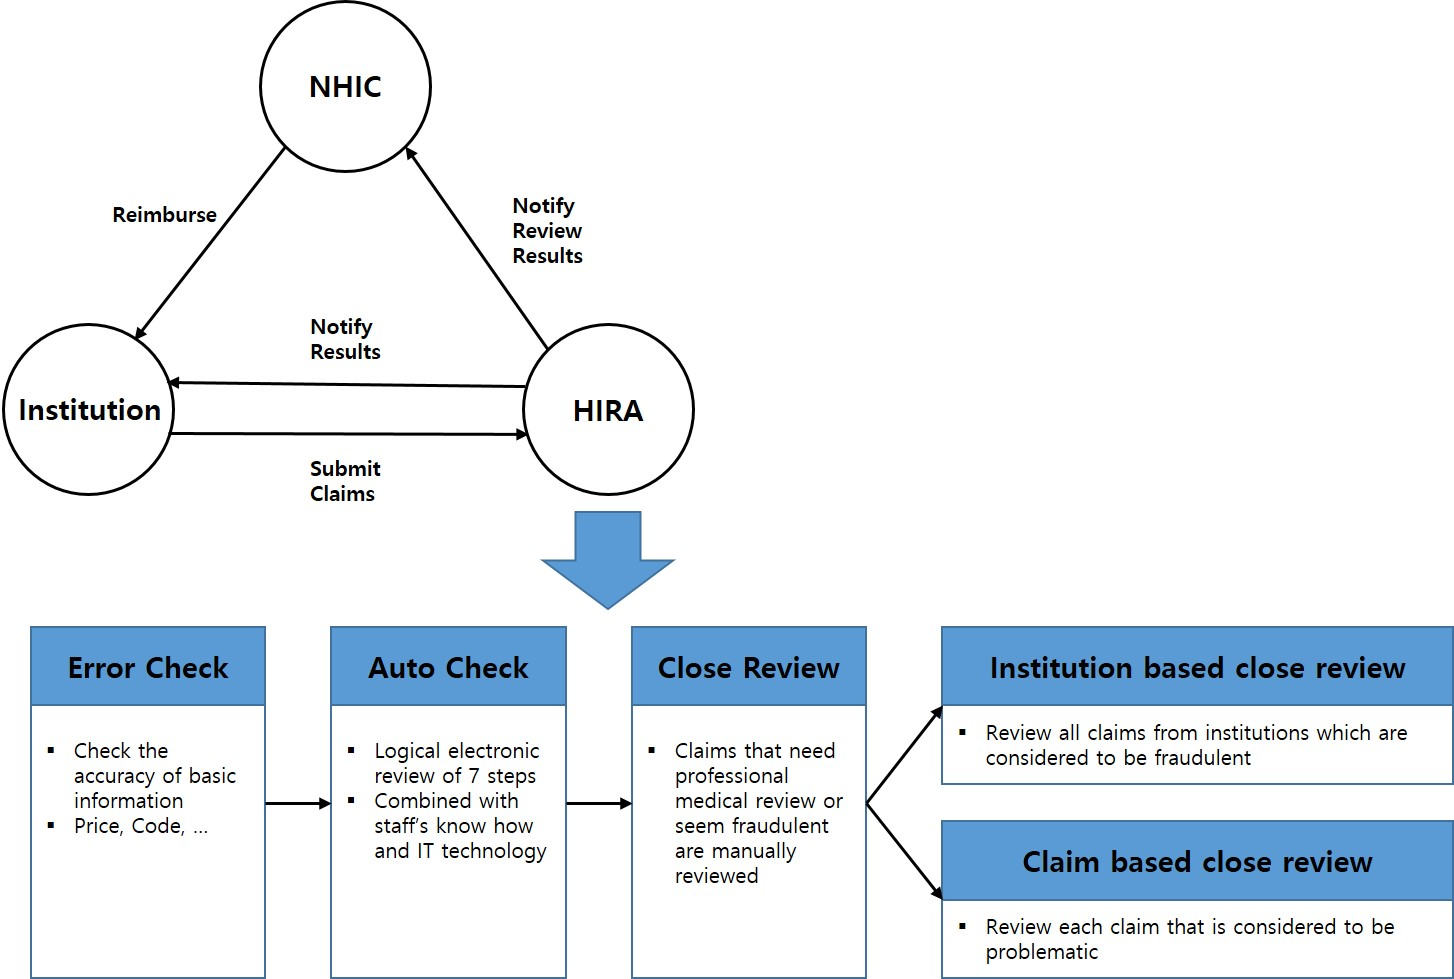
\includegraphics[width=0.9\textwidth]{[figure1]HIRA_review_process.jpg}
   \vspace{-0.5cm}
   \caption{요양 기관의 청구 명세서 접수, 변제 및 HIRA의 심사 프로세스: medical institution에서 HIRA에 청구명세서를 접수하면, HIRA의 review process를 거쳐, 이를 NHIC에 통보하고, 이를 기반으로 NHIC에서는 해당institution에게 변제해준다.}
   \vspace{0.5cm}
   \label{fig:review process}
\end{figure}

요양 기관에서 HIRA에 청구명세서를 접수하면, 각 청구명세서의 환자 질병 코드, 청구 코드나 가격 오류, 기록 누락 여부 등에 대한 전산 점검(Error check)이 이루어진다.
그 후, 심사자들의 심사 관련 지식들을 갖고 있는 HIRA 내의 심사 프로그램으로 모든 청구명세서에 대해서 심사하는, 전산 심사(auto check)과정을 거치게 된다.
이 과정에서는 비교적 간단한 항목들에 대해서 7단계에 걸쳐서 심사를 한다.
이러한 과정을 통과한 청구명세서는, 일부는 전문 심사(close review)과정을 거치게 되고, 잔여분에 대해서는 해당 요양기관에 정상적으로 변제해준다.

전문 심사는 착오 청구 개연성이 높거나 전문 의학적 판단이 필요한 청구명세서에 대해서 심사관들이 직접 심사하는 것이다.
일차적으로 심사 직원에 의한 심사가 이루어지고, 전문 의학적 판단을 위해 해당분야 전문의사가 하는 심사위원 심사와 여러 전문가가 모여서 적정성 여부를 심사하는 심사위원회 심사를 수행한다.
이 때, 전문 심사는 다음과 같이 2가지의 심사를 병행하여 이루어 진다.

\begin{itemize}
\item 기관 단위 전문 심사: Fraudulent 기관을 선정하고, 해당 기관의 모든 명세서를 심사하는 방법으로, 기관 선정을 잘 하는 것이 매우 중요하다.
현재 HIRA에서는 기관의 총 진료비, 환자 당 평균 진료비 등 기관 단위의 변수를 추출하여 HIRA내부에서 개발된 기관 선정 모형에 input으로 넣으면, 기관의 fraudulent score가 계산되는데, 이 score가 높은 기관들을 일부 선정한다.
이와 더불어, 심사가 필요하다고 판단되는 기관들을 HIRA내의 추가 규칙에 의해 선정한다.
\item 건 단위 전문 심사: HIRA에 접수된 청구 명세서 중, 기관 단위 전문 심사와 별도로, 특별히 심사가 필요하다고 여겨지는 명세서나, 환자의 전체 명세서, 혹은 신생 의료 기관에서 청구한 전체 명세서에 대해서 수시로 심사하는 방법이다.
\end{itemize}

본 연구에서는 위의 심사 방법들 중, 기관 단위 전문 심사 방법을 개선하였다.
기관 단위 전문 심사의 성공 여부는 심사의 대상이 되는 기관을 잘 선정하는 것에 달려있다.
심사 대상 기관이 잘 선정될 경우, 해당 기관에는 조정 대상이 되는 fraudulent 진료 내역이 많아서, 현실적으로 제한된 심사량 대비 많은 사기 진료 내역을 탐지할 수 있다.
그러나, 기관을 잘못 선정할 경우에는 사기 진료 내역을 많이 탐지하지 못하여 매우 비효율적인 심사를 할 수 밖에 없다. 

그러나 기존에 HIRA에서 사용하던 모형에서 활용하는 변수들은 각 청구명세서 혹은 기관의 총 환자 수, 한 환자의 평균 내원 횟수 같은 기관 단위의 정보만을 활용하기 때문에, 정보들이 aggregate되어 진료 내역 단위의 자세한 정보들이 누락되게 된다.
뿐만 아니라, 해당 모형은 예전에 개발된 것으로 현재 의료 상황과는 맞지 않는 부분이 있고, fraud 형태가 점점 더 복잡해짐에 따라, 기존 모형으로는 detect하지 못하는 경우들이 많아져, 효율적인 기관 선정이 이뤄지지 못하고 있다.
이를 극복하기 위해, HIRA에서는 기존 모형에 별도의 추가 규칙으로 기관을 선정하고 있다.
그러나, 이런 방법으로도 fraudulent한 청구명세서를 많이 탐지하지 못하고 있어, 의료 기관들의 fraudulent billing으로 발생하는 사회 경제적 낭비를 충분히 줄이지 못하고 있다. 

\section{Proposed method}
\label{3}
\subsection{Modeling}
\label{3.1}
\subsubsection{Modeling step 1: medical treatment-based model}
\label{3.1.1}

진료 내역 단위 모델은 기본적으로 인공 신경망 기반의 모델로, 진료 내역의 정보들을 입력 변수로 하여, 해당 내역이 fraudulent할 score를 산출한다.
이 때, input 변수에는 나이, 성별, 질병 등 수진자와 관련된 정보들과, 투약일수, 진료 행위 등 진료 내역과 관련된 정보들이 포함되어 있다.
전체적인 모델 구조는 그림~\ref{fig:model structure}와 같다.

\begin{figure}[h]
   \centering
   \vspace{0.5cm}
   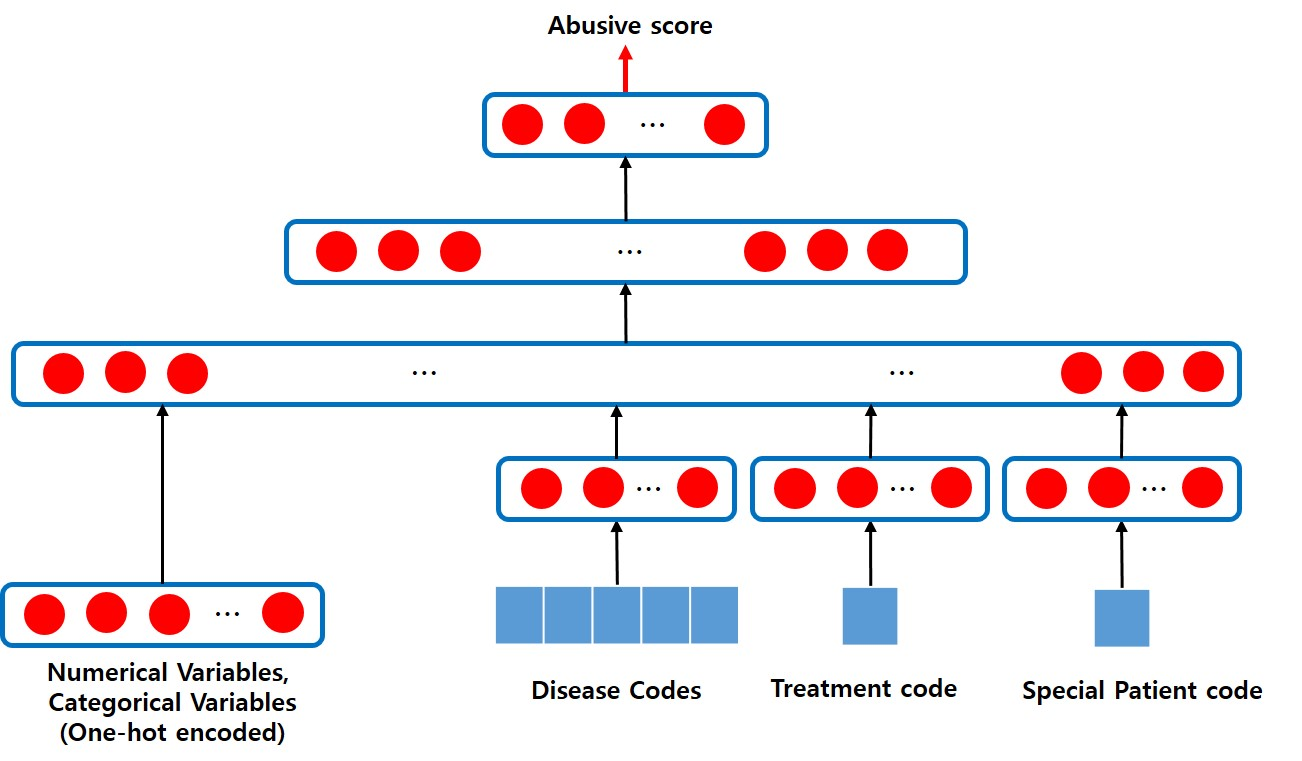
\includegraphics[width=0.9\textwidth]{[figure2]network_structure.jpg}
   \vspace{-0.5cm}
   \caption{진료 내역 단위 모델. 범주의 갯수가 많은 범주형 변수의 경우, embedding하여 vectorize하여, 전체 변수들을 concatenate}
   \vspace{0.5cm}
   \label{fig:model structure}
\end{figure}

모델링에 사용하는 변수들은 수치형 변수와 범주형 변수가 같이 존재하는 heterogeneous data이다.
일반적으로는 입력 변수의 type을 맞춰주기 위해서, 일반적으로 범주형 변수들에 대해 one-hot encoding과정을 통해 수치형 변수로 변환하는 과정을 수행한다.
그러나, 이러한 방법은 범주의 개수가 적은 변수에는 사용할 수 있지만, 범주의 개수가 많은 변수에 이 방법을 적용할 경우 데이터의 차원이 매우 커지게 되어 적합하지 않다.
본 연구에서 사용한 데이터에서도, 이러한 범주형 변수가 존재하여, one-hot encoding 방법을 적용시킬 수 없다.
그 대신, 이러한 변수들은 numerical space에 embedding시켜서 numeric vector로 변환하였다.
이 때, 이 embedding function도 전체 모델이 학습되면서 같이 학습된다.

위와 같은 변수들의 embedding방법은 다음과 같다. 어떤 범주형 변수에 대해서, 범주의 갯수는 $V$개이고, 해당 변수를 $d \ll V)$ 차원의 공간에 embedding하고자 한다.
Embedding matrix $\mathbf{W}$가 있을 때, One-hot encoded vector $\mathbf{x} = [x_1, x_2, ..., x_V]$ 의 embedded vector $\mathbf{h}$ 는 다음과 같이 계산된다.

$$\mathbf{h} = f(\mathbf{x}) = \mathbf{x^T}\mathbf{W}$$

이 때, embedding matrix $\mathbf{W} \in\mathbf{R}^{V \times D}$도 이분류 인공신경망을 학습하면서 같이 학습이 되는데, 전체 인공신경망의 error를 최소화하도록 학습이 진행된다.
본 연구에서의 목적인 이분류 인공신경망의 경우, binary cross entropy function을 사용하여 다음과 같이 정의된다.

$$\mathbf{L} = -\sum_{i=1}^N(y_i\log\hat{y_i} + (1-y_i)\log(1-\hat{y_i})$$

인공신경망의 학습 방법인 error backpropagation을 진행할 때, 전체 인공신경망뿐만 아니라, embedding matrix $\mathbf{W}$에도 error를 backpropagate하여, 분류 error를 최소화 하는 방향으로 범주형 변수들을 embedding시킬수 있도록 $\mathbf{W}$를 학습시킨다.

\begin{figure}[h]
   \centering
   \vspace{0.5cm}
   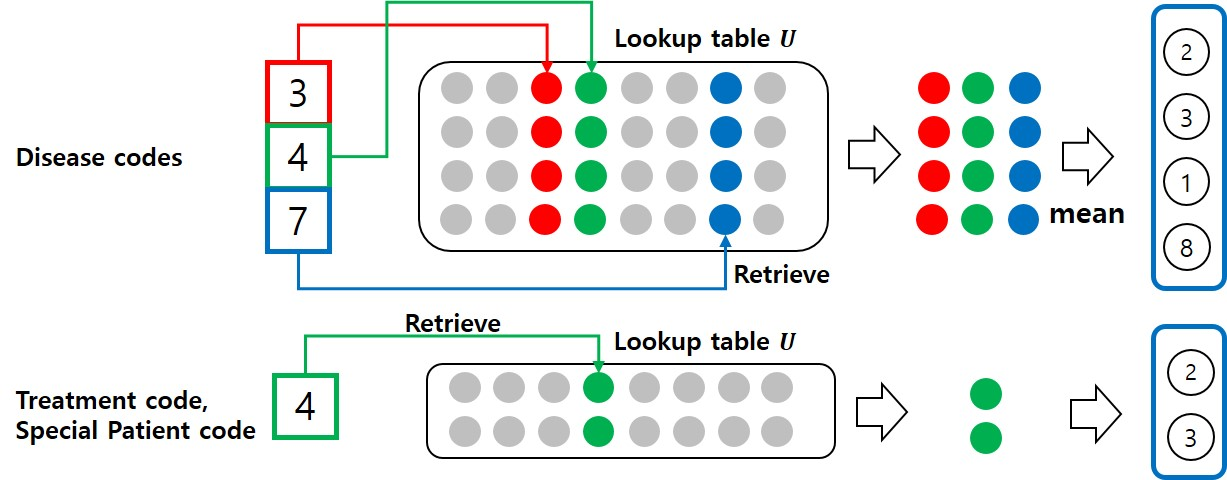
\includegraphics[width=0.9\textwidth]{[figure3]embedding_method.jpg}
   \vspace{-0.5cm}
   \caption{범주형 변수의 embedding 방법.(Up): 하나의 진료 내역에 여러 개의 범주가 공존하는 변수의 embedding 방법으로, diangnosis code가 이에 해당함.(down): 하나의 진료 내역에 하나의 범주만 존재하는 변수의 embedding방법으로, treatment code, special patient code가 이에 해당함}
   \vspace{0.5cm}
   \label{fig:category embedding method}
\end{figure}


여기서 한가지 더 고려해야 할 것은, 환자의 질병 정보이다.
일반적으로 환자는 한 개의 질병을 갖고 있는 경우보다, 여러 개의 질병을 앓고 있는 경우가 많다.
이런 경우, 이상적으로 환자의 질병과 의사의 진료 내역 간의 명확한 인과관계에 대한 정보가 데이터에 있는 것이 좋다.
그러나, 실제로 의사가 수행하는 진료 행위나 처방하는 약제들은 하나의 질병에 기인하기 보다는, 환자가 갖고 있는 질병을 종합적으로 고려하여 수행하는 경우가 많다.
이러한 이유로 인해, HIRA에 접수되는 청구명세서에는 각 진료 내역이 어떤 질병에 의해 수행되어 있는가에 대한 mapping이 되어 있지 않다.
그 대신, 각 진료 내역은 모든 질병과 mapping이 되어 있다.
이러한 환자의 질병 데이터를 수치형 변수로 변환하기 위해 그림~\ref{fig:category embedding method}과 같이 각 질병 코드에 대해서 각각 embedding하고, 이를 나중에 average하는 방식으로 환자의 질병 내역들을 embedding하였다.
이와 같은 방법으로 하나의 진료 내역에 대해서 모든 질병 내역을 종합적으로 고려할 수 있도록 하였다.

\subsubsection{Modeling step 2: fraudulent기관 선정 방법}
\ref{3.1.1}에서 학습한 모델은 각 진료 내역이 사기일 score를 산출해 낸다.
이를 기반으로 다음과 같이 기관의 fraudulent billing pattern이 나타나는 정도를 scoring 하는 방법인 Treatment based Fraudulent Institutes Detection(TFID)방법론을 제안한다. 
이를 도식화 하면 그림~\ref{fig:whole process}와 같다.

\vspace{5mm}
\noindent\fbox{%
    \parbox{\textwidth}{%
    \vspace{3mm}
        $N$개의 기관이 있고, 각 기관에는 $n_1, n_2, \dots, n_N$개의 medical treatments가 있다고 하자.
        
        기관 $i$의 진료 내역에 대한 청구금액을 각각 $c_{i1}, c_{i2}, \dots, c_{ik}, \dots, c_{in_i}$라고 하고, \ref{3.1.1}에서 학습된 모델로 이들에 대해서 scoring한 fraudulent score를 $\hat{y}_{i1}, \hat{y}_{i2}, \dots, \hat{y}_{ik}, \dots \hat{y}_{in_i}$라고 하자.
        이 때, 기관의 fraudulent billing을 갖는 정도를 나타내는 TFID score는 다음과 같이 계산된다.
        
        \begin{itemize}
        \item (step1): 진료 내역별 기대 조정 금액 산출($m_{ik}$)
        $$m_{ik} = c_{ik} \times \hat{y}_{ik}$$
        \item (step2): 기관별 기대 조정 금액 산출($M_i$)
        $$M_i=\sum_{k=1}^{n_i}m_{ik}$$
        \end{itemize}
        for $k = 1,2,\dots, n_i, i=1,2,\dots,N$
    \vspace{3mm}
    }%
}

\vspace{5mm}

위에서 계산된 기관별 기대 조정 금액인 $M_i$를 기관의 fraudulent score인 TFID score로 정의하고, 이 score가 높은 상위 기관들을 fraudulent 기관으로 선정한다.
청구 금액을 같이 고려함으로써, fraudulent score가 비슷한 진료내역이라도, 기대 utility가 높은 진료 내역을 우선으로 탐지함으로서, 심사의 효율성을 극대화 할 수 있다.

\begin{figure}[h]
   \centering
   \vspace{0.5cm}
   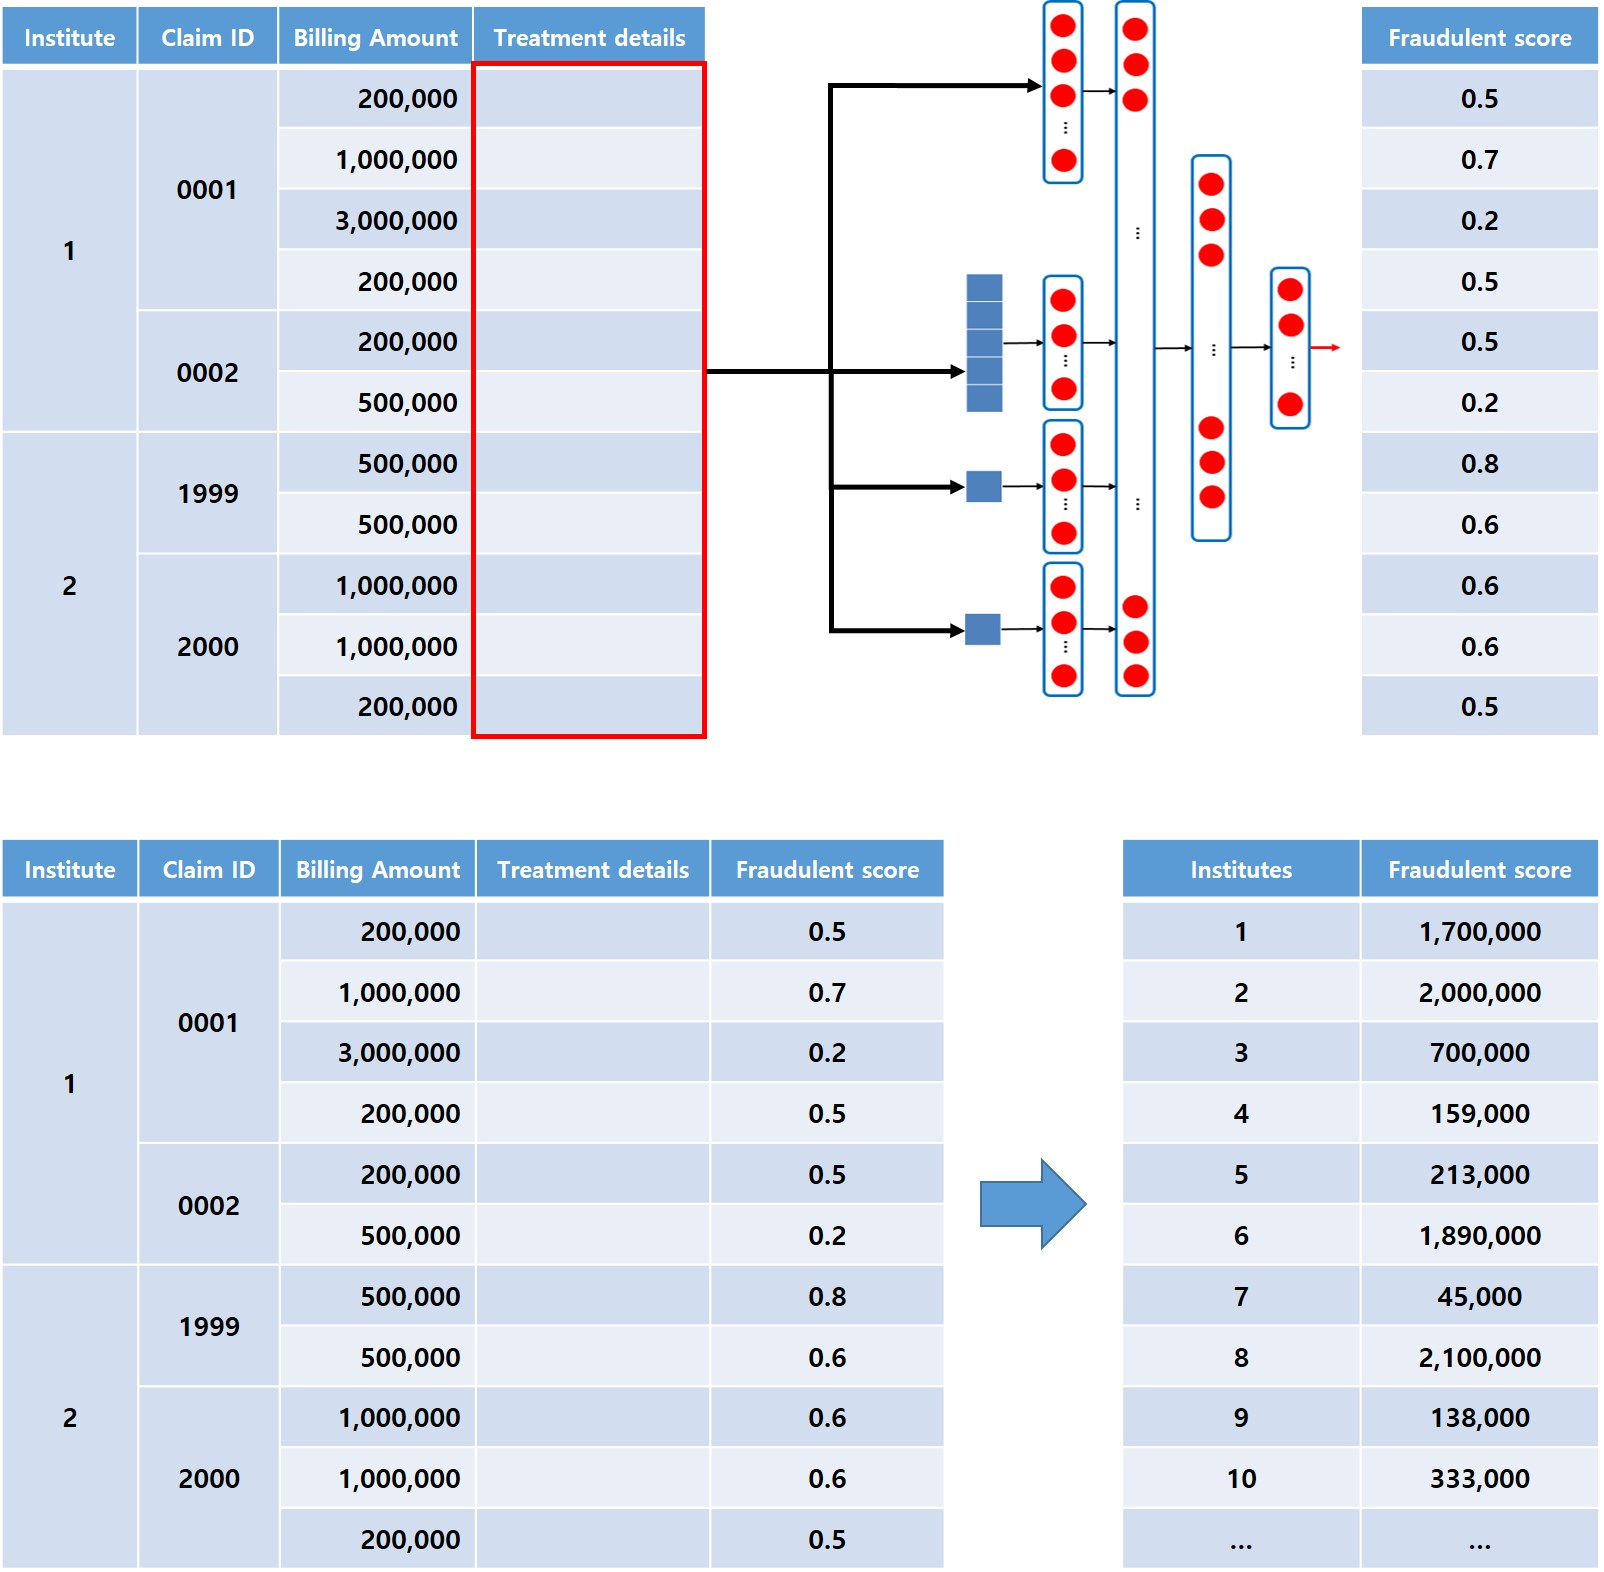
\includegraphics[width=0.7\textwidth]{[figure4]TFID_score_process.jpg}
   \vspace{-0.5cm}
   \caption{전체 프로세스.(Up): 학습된 treatment-based scoring model에 대해서, 각 내역에 대해서 fraudulent score를 계산. (down): treatment내역의 정보와 해당 내역의 fraudulent score로 기관의 fraudulent한 정도를 나타내는 TFID score를 계산하는 과정}
   \vspace{0.5cm}
   \label{fig:whole process}
\end{figure}


\subsection{모델의 효율성 평가 방법}
\label{3.2}
이 절에서는 효율성의 향상을 quantify하고 얼마나 향상했는지를 측정하는 relative efficiency와 precision@k term에 대해서 소개한다.
이를 통해, TFID모델이 기존에 사용하던 모델보다 더 우수하다는 것을 보인다.

\subsubsection{Relative Efficiency}
\label{3.2.1}

그림~\ref{fig:relative efficiency1}의 왼쪽 그림은 전문 심사를 수행한 기관들을 모델 A와 모델 B로 평가했을 때의 fraudulent score와 각 기관의 실제 조정 금액을 나타낸 것이다.
여기서, 실제 조정 금액이라는 것은 심사자들이 실제로 기관의 모든 진료 내역에 대해서 심사하고, 의료 기관이 이 금액만큼 과다하게 청구했다는 것을 의미한다.
즉, 이 금액은 기관의 실제 fraudulent billing이다.
만약, 모델이 잘 학습되었다면 기관의 조정 금액과, score가 비례 관계에 있어야 할 것이다.
이를 고려하였을 때, 기관의 fraudulent billing pattern은 모델 A보다는 모델 B가 더 잘 scoring한다고 할 수 있다.
이 때, 실제로 모델 A score가 높은 순서대로 심사를 했을 때와, 모델 B score가 높은 순서대로 심사했을 때의 실제 누적 조정 금액을 도식화 한 것이 그림~\ref{fig:relative efficiency1}의 오른쪽 그림이다.
만약, 심사하는 기관의 수를 지금의 절반이라고 생각해보자.
위의 그림에 따르면, 모델 A score대로 심사 기관을 선정하였을 때, 실제 누적 조정 금액은 현재의 절반 가량밖에 안되는 반면, 모델 B score대로 심사 기관을 선정하였을 경우, 실제 누적 조정 금액은 현재의 80\%가량인 것을 볼 수 있다.
즉, 모델 B score를 기반으로 심사 대상 기관을 선정할 때, 좀 더 효율적인 심사를 할 수 있게 된다.

\begin{figure}[h]
   \centering
   \vspace{0.5cm}
   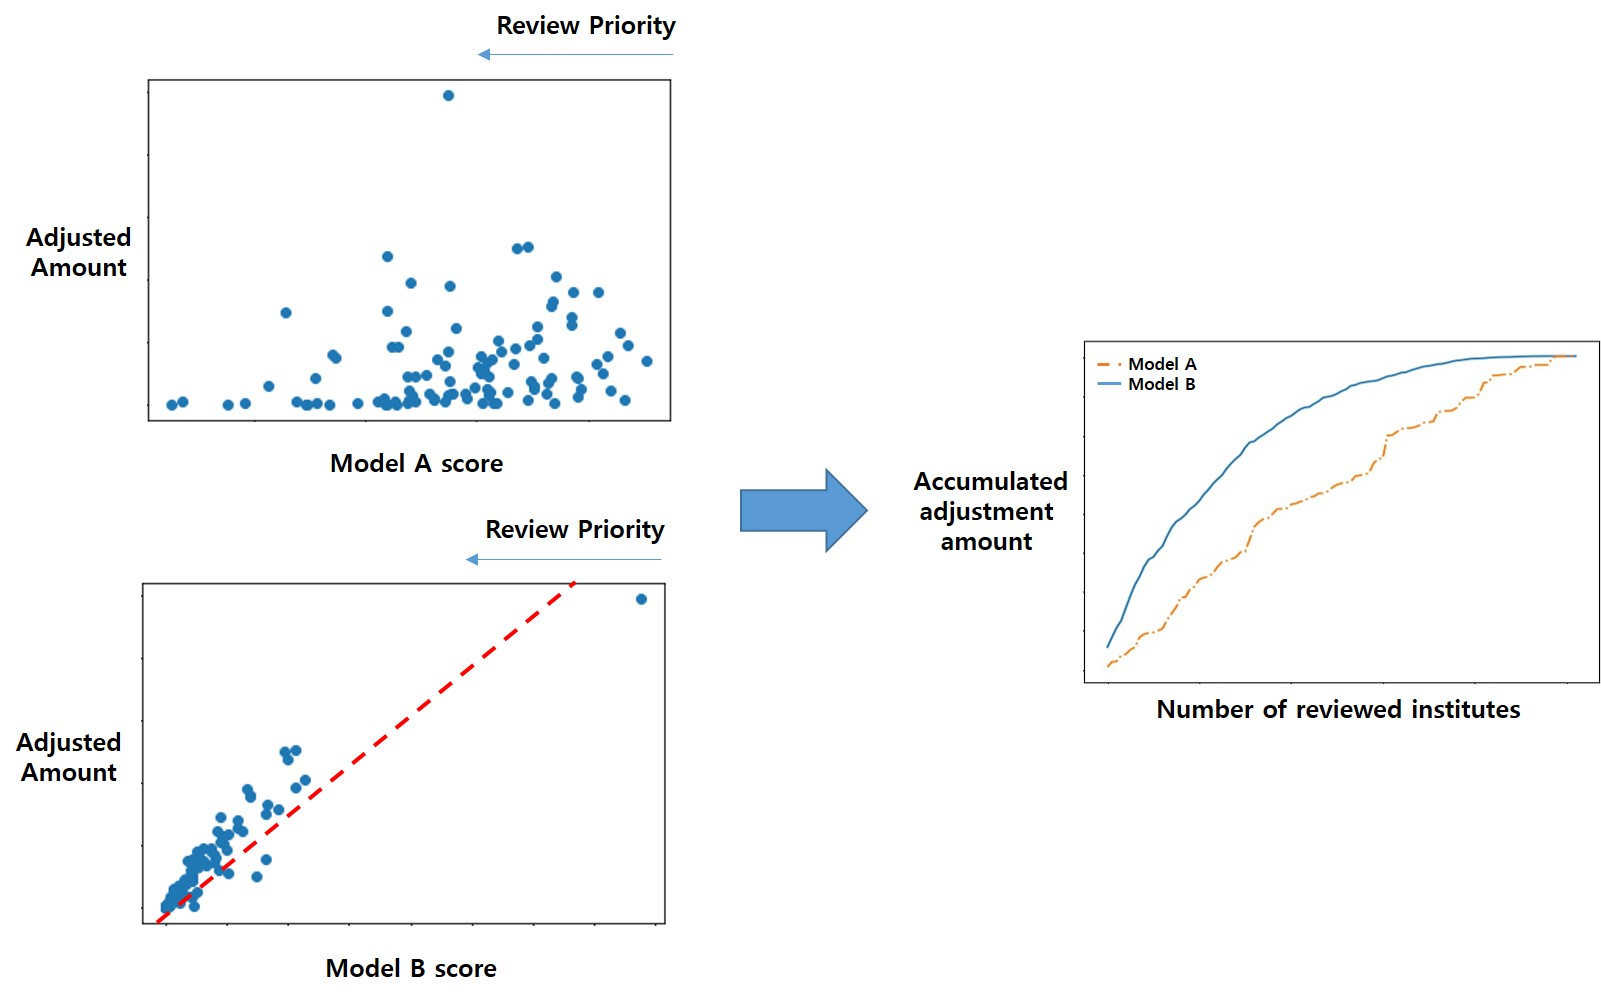
\includegraphics[width=0.9\textwidth]{[figure5]relative_efficiency1.jpg}
   \vspace{-0.5cm}
   \caption{(left): 각 기관의 실제 조정 금액과 해당 기관들에 대해 모델 A,B가 매기는 score (right): 각 모델의 상위 score순으로 실제로 review하였을 때, 실제 누적 조정 금액}
   \vspace{0.5cm}
   \label{fig:relative efficiency1}
\end{figure}

여기서 모델의 효율성에 대해서 좀 더 정교하게 정의해보자.
심사에 필요한 노력 대비, 실제 누적 조정 금액을 모델의 효율성이라고 할 수 있다.
이제까지 심사에 필요한 노력은 심사한 기관 수로 생각해 왔다.
그러나, 기관마다 거의 동일한 양의 심사명세서를 청구하면 이렇게 생각해도 괜찮으나, 실제로는 기관마다 청구명세서의 양이 다르다.
그렇기 때문에, 심사하는 비용은 기관마다 다를 수 있다.
그렇기 때문에 심사에 필요한 비용을 심사하는 기관 수가 아닌, 실제로 심사하는 청구명세서 수로 정교하게 정의할 필요가 있다.
즉, n개의 청구 명세서를 심사할 때, 실제 조정 금액을 심사의 효율성이라고 할 수 있다.
그림~\ref{fig:relative efficiency2}와 같이 누적 청구 명세서 수와 누적 조정 금액을 같이 고려해 줘야 한다.
이를 수식으로 정의하면 다음과 같다.

\begin{figure}[h]
   \centering
   \vspace{0.5cm}
   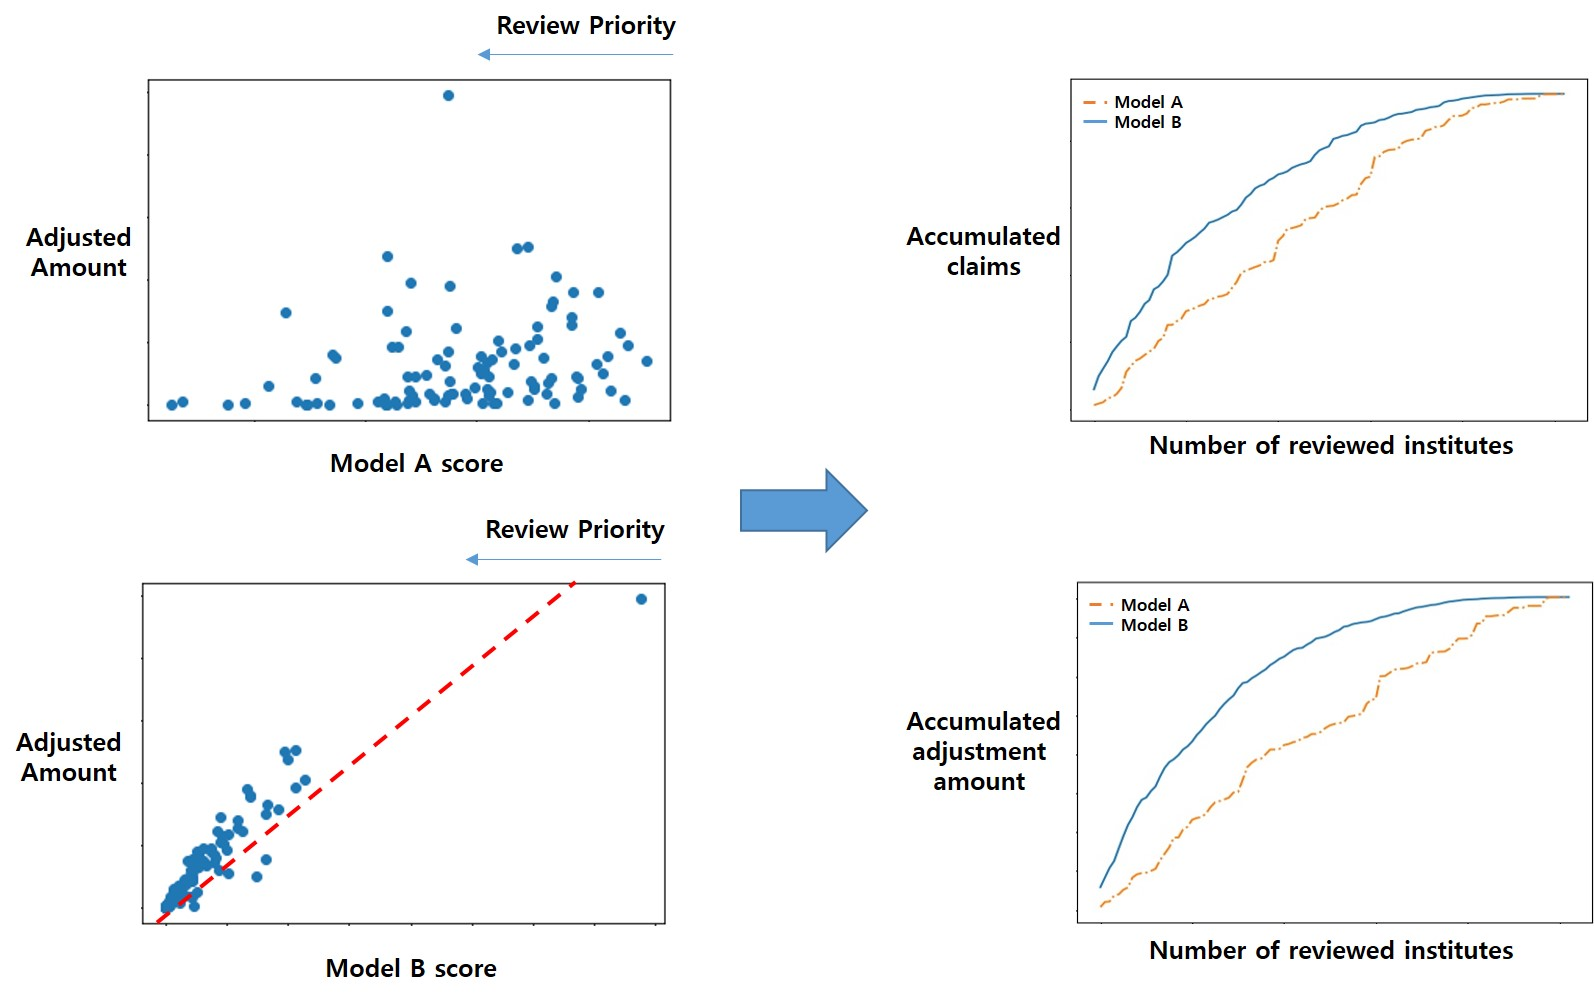
\includegraphics[width=0.9\textwidth]{[figure6]relative_efficiency2.jpg}
   \vspace{-0.5cm}
   \caption{(left): 각 기관의 실제 조정 금액과 해당 기관들에 대해 모델 A,B가 매기는 score (right): 각 모델의 상위 score순으로 실제로 review하였을 때, 누적 청구명세서 수와 실제 누적 조정 금액}
   \vspace{0.5cm}
   \label{fig:relative efficiency2}
\end{figure}

여기서, 우리는 데이터의 보안 issue상 절대적인 금액이나 efficiency를 보여줄 수 없기 때문에, relative efficiency를 정의하여 모델 A와 B의 효율성을 비교하는 척도로 삼는다.
이를 통해, 모델 A의 score로 기관을 선정할 때보다, 모델 B의 score로 기관을 선정하였을 때의 향상된 심사 효율성을 정량화할 수 있다.

본 연구에서는 심사할 청구명세서의 양을 정해놓지 않고, 전체에서 얼마나 심사할지를 변화시키면서 이 효율성을 볼 것이다.
이는 본 연구에서는 진료 과목별로 별도의 모델을 만들고, 진료 과목마다 청구되는 청구 명세서 수가 다르기 때문이다.
또한, 본 연구에서는 기존 모형 대비 TFID모형을 비교하므로, relative efficiency는 다음과 같이 정의한다.

\subsubsection{precision@k}
\label{3.2.2}

precision at k는 일반적으로 다음과 같이 정의된다.
\[
 \text{precision@k} = \frac{\text{number of recommended items at k that are relevant}}{\text{number of recommended items at k}}
\]
% $$\frac{number of recommended items at k that are relevant}{number of recommended items at k}$$

즉, k개의 item을 retrieve했을 때, 그 중에서 실제로 목표했던 것과 relevant한 비율이다.
본 연구에서는 이러한 정의를 응용하여, 이를 다음과 같이 정의한다.
전체 기관들 중, TFID가 높은 k\%의 기관을 심사한다고 할 때, 실제 조정 금액도 상위 k\%에 속하는 기관의 비율을 precision@k로 정의한다.
이 measure도 실제 조정 금액과 기관의 fraudulent score간의 상관관계를 나타낸다.
특히, k값이 작을 때의 precision@k는 fraudulent billing pattern이 심각하게 나타나는 기관들을 모델이 얼마나 detect할 수 있는 가를 나타낸다.
이를 수식으로 나타내면 다음과 같다.

\[
 \text{precision@k} = \frac{\text{number of institutions that has both top k\% adjusted amount and model score}}{\text{number of institutions that has top k\% model score}}
\]

\section{Experiment}
\label{4}
\subsection{Data}
\label{4.1}

본 연구에서는 2016년동안 ‘병원’급에서 발생한 진료 내역들 중, 총 6개의 진료과목(정형외과, 신경외과, 소아청소년과, 재활의학과, 외과, 신경과)의 입원 환자 진료 내역 데이터를 기반으로 전문 심사 대상 기관을 선정하는 모델을 개발한다.
이를 위해, [Table1]에 있는 data들을 그림~\ref{fig:integrated data}와 같이 통합하고, 이를 모델링에 활용한다.

% Please add the following required packages to your document preamble:
% \usepackage{booktabs}
\begin{table}[]
    \centering
    \caption{사용한 database목록}
    \vspace{0.5cm}
    \label{table: table information}
    \begin{tabular}{@{}ll@{}}
    \toprule
    \multicolumn{1}{c}{Table}                 & \multicolumn{1}{c}{상세 내역} \\ \midrule
    Claim information     & \begin{tabular}[c]{@{}l@{}}- claim의 기본 정보\\ - claim ID, 환자 기본 정보, 요양일수 등\end{tabular}       \\ \midrule
    Treatment details     & \begin{tabular}[c]{@{}l@{}}- 명세서 별 진료 내역 정보 및 처방 정보\\ - 진료 행위, 청구 금액, 약제 사용량 등\end{tabular} \\ \midrule
    Review details        & \begin{tabular}[c]{@{}l@{}}- 진료 내역의 조정 정보\\ - 조정 발생 여부, 조정된 금액 등\end{tabular}               \\ \midrule
    Diagnosis information & \begin{tabular}[c]{@{}l@{}} - 각 claim에 해당하는 환자의 질병 내역\end{tabular}                                                               \\ \bottomrule
    \end{tabular}
\end{table}


\begin{figure}[h]
   \centering
   \vspace{0.5cm}
   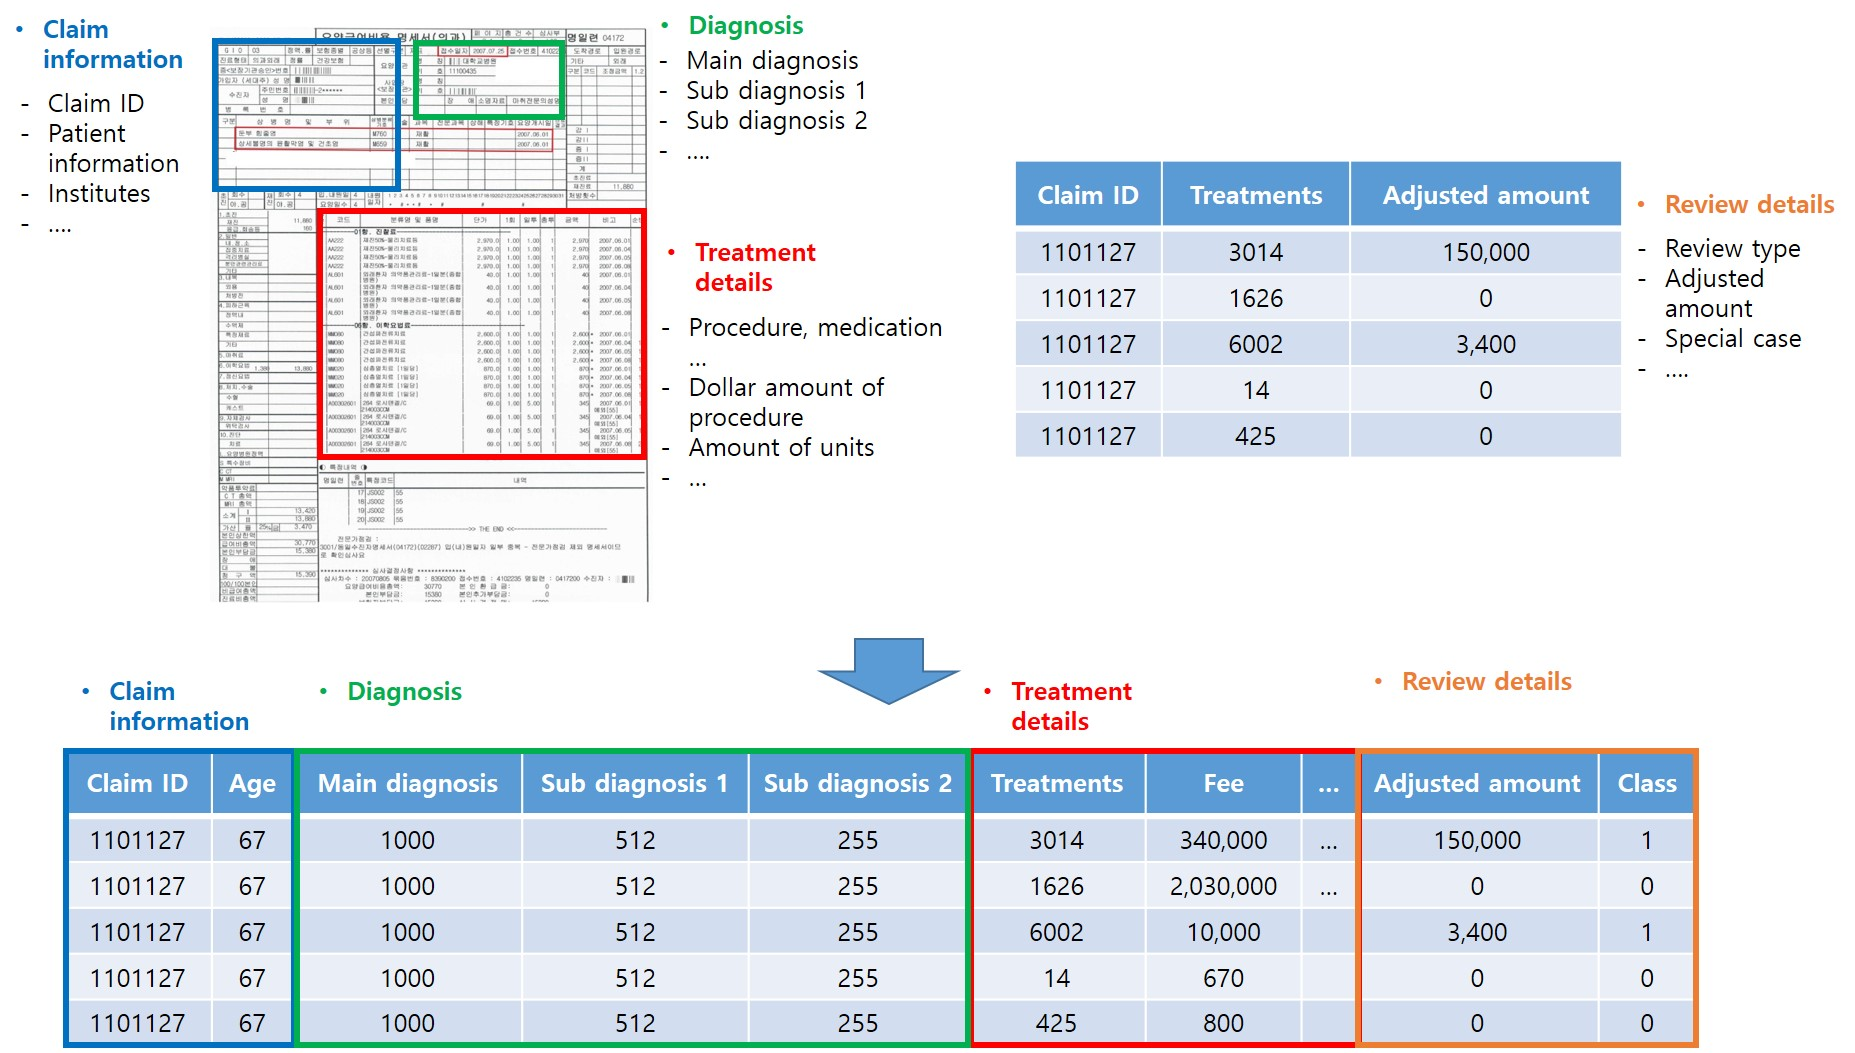
\includegraphics[width=0.9\textwidth]{[figure7]integrated_data.jpg}
   \vspace{-0.5cm}
   \caption{실제 청구 명세서에서 각 database에 저장되는 정보에 해당하는 내용들과, review deails에 대한 정보를 통합하여, 모델링에 사용하는 통합 데이터 형태}
   \vspace{0.5cm}
   \label{fig:integrated data}
\end{figure}


모든 기관들은 심사 유형을 기준으로 할 때, 3가지 종류로 나눌 수 있다: (1) full close review, (2) partial close review, (3): full auto check.
Full close review에 해당하는 기관들은 fraudulent 기관으로 선정이 되어서, 심사자들이 해당 기관에서 청구한 청구명세서들은 전부 심사하는 경우이다.
Full auto check에 해당하는 기관들은, fraudulent가 거의 없다고 판단되어, auto check로 기본적인 사항들에 대해 심사하고, 심사자들의 manual 심사는 없는 기관들이다.
Partial close review에 해당하는 기관들은, 기관 자체는 fraudulent한 기관으로 선정되지는 않으나, 심사자들이 개별 청구명세서, 혹은 개별 환자의 전체 명세서들을 심사한 경우로, 일부만 심사자들의 manual 심사가 이루어지고, 나머지는 auto check만 하는 기관들이다.
표~\ref{table: review statistics}는 진료과목 별로 각 case들이 얼마나 있는지를 나타낸 것이다.
본 연구의 목표는 심사자들의 심사 logic을 학습한 모델을 구축하는 것이기 때문에, full close review 기관의 전체 청구명세서와 partial close review 기관 중에서, manual 심사가 이루어진 청구명세서들을 활용하였다. 

% \usepackage{booktabs}
% \usepackage{multirow}
\begin{table}[]
\centering
\caption{각 진료과목 case별 기관 수, 청구명세서 수, treatment 수}
\vspace{0.5cm}
\label{table: review statistics}
\begin{tabular}{@{}ccccc@{}}
\toprule
Department                                                                                   & Review type                           & \begin{tabular}[c]{@{}c@{}}Number of\\ institutions\end{tabular} & \begin{tabular}[c]{@{}c@{}}Number of\\ claims\end{tabular} & \begin{tabular}[c]{@{}c@{}}Number of\\ treatments\end{tabular} \\ \midrule
\multirow{4}{*}{\begin{tabular}[c]{@{}c@{}}Orthopedics\\ (정형외과)\end{tabular}}                & Autocheck                             & 9                                                                & 14                                                         & 656                                                            \\ 
                                                                                             & \multirow{2}{*}{Partial close review} & \multirow{2}{*}{422}                                             & 295,208(close)                                             & 16,270,697(close)                                              \\
                                                                                             &                                       &                                                                  & 92,494(auto)                                               & 6,456,933(auto)                                                \\ 
                                                                                             & Full close review                     & 393                                                              & 525,303                                                    & 42,025,970                                                     \\ \midrule
\multirow{4}{*}{\begin{tabular}[c]{@{}c@{}}NeuroSurgery\\ (신경외과)\end{tabular}}               & Autocheck                             & 7                                                                & 9                                                          & 227                                                            \\ 
                                                                                             & \multirow{2}{*}{Partial close review} & \multirow{2}{*}{159}                                             & 44,962(close)                                              & 3,194,142(close)                                               \\
                                                                                             &                                       &                                                                  & 19,090(auto)                                               & 1,177,614(auto)                                                \\ 
                                                                                             & Full close review                     & 255                                                              & 283,444                                                    & 20,928,502                                                     \\ \midrule
\multirow{4}{*}{\begin{tabular}[c]{@{}c@{}}Pediatrics\\ (소아청소년과)\end{tabular}}               & Autocheck                             & 15                                                               & 5,528                                                      & 44,740                                                         \\ 
                                                                                             & \multirow{2}{*}{Partial close review} & \multirow{2}{*}{248}                                             & 123,842(close)                                             & 7,567,527(close)                                               \\
                                                                                             &                                       &                                                                  & 352,838(auto)                                              & 15,022,869(auto)                                               \\ 
                                                                                             & Full close review                     & 33                                                               & 30,412                                                     & 2,029,174                                                      \\ \midrule
\multirow{4}{*}{\begin{tabular}[c]{@{}c@{}}Rehabilitation\\ Medicine\\ (재활의학과)\end{tabular}} & Autocheck                             & 0                                                                & 0                                                          & 0                                                              \\  
                                                                                             & \multirow{2}{*}{Partial close review} & \multirow{2}{*}{81}                                              & 62,591(close)                                              & 2,414,527(close)                                               \\
                                                                                             &                                       &                                                                  & 9,248(auto)                                                & 328,500(auto)                                                  \\ 
                                                                                             & Full close review                     & 103                                                              & 102,703                                                    & 4,527,046                                                      \\ \midrule
\multirow{4}{*}{\begin{tabular}[c]{@{}c@{}}General\\ Surgery(외과)\end{tabular}}               & Autocheck                             & 20                                                               & 187                                                        & 6,111                                                          \\  
                                                                                             & \multirow{2}{*}{Partial close review} & \multirow{2}{*}{273}                                             & 40,716(close)                                              & 2,612,109(close)                                               \\
                                                                                             &                                       &                                                                  & 34,521(auto)                                               & 1,772,117(auto)                                                \\  
                                                                                             & Full close review                     & 156                                                              & 38,024                                                     & 2,404,017                                                      \\ \midrule
\multirow{4}{*}{\begin{tabular}[c]{@{}c@{}}Neurology\\ (신경과)\end{tabular}}                   & Autocheck                             & 17                                                               & 62                                                         & 3,387                                                          \\ 
                                                                                             & \multirow{2}{*}{Partial close review} & \multirow{2}{*}{102}                                             & 17,236(close)                                              & 1,054,902(close)                                               \\
                                                                                             &                                       &                                                                  & 4,347(auto)                                                & 258,345(auto)                                                  \\  
                                                                                             & Full close review                     & 116                                                              & 33,462                                                     & 2,136,354                                                      \\ \bottomrule
\end{tabular}
\end{table}


인공신경망 기반의 scoring 모델링을 하기 위해서는 class에 대한 정의가 필요하다.
진료 내역 자체가 불필요하다고 판단되는 경우, 해당 진료 내역의 청구 금액 전체가 조정 금액이 되기도 하며, 일부가 과다하게 청구되었다고 판단되는 경우, 청구 금액 중에서 일부만 이에 해당하기도 한다.
본 연구에서는 조정 금액이 일부라도 발생한 경우를 normal, 그렇지 않은 경우를 fraud이라고 정의한다. 

필요한 변수 선택, 모델링 대상 진료 과목에 해당하는 진료 내역 선택, missing value 제거, 데이터 오류 제거 등 일련의 전처리 과정을 통해, 모델링에 적합한 형태로 약 110M개의 데이터를 추출하였다.
또한 사용하는 변수들은 청구 금액을 포함한 18개의 수치형 변수와 18개의 범주형 변수이다.
어떤 변수를 사용하였는가에 대한 내용은 데이터의 보안 문제로 인하여 여기서 따로 자세하게 밝히지는 않는다.
범주형 변수에는 질병 코드, 특정 환자구분코드, 진료 코드가 포함되어 있는데, 각각 1,902개, 196개, 7,882개의 범주 값을 갖는다.
또한, \ref{3.1.1}에서 언급했던 것과 같이 각 진료 내역은 한 개의 특정 환자구분코드, 진료 코드를 갖고 있으나, 질병 코드는 최대 30개의 질병 코드를 갖고 있다.
추출된 데이터로 모델링을 하기 위해, 각 set의 분포가 최대한 동일하게 유지되도록 하면서 (training) : (validation) : (test)의 비율을 6:2:2가 되도록 나누었다.
표 ~\ref{table: data split}에 이러한 과정을 수행하고 모델링에 사용한 dataset의 최종 개수를 나타낸 표를 포함하였다.

\begin{table}[]
    \centering
    \caption{Training - Validation - Test set}
    \vspace{0.5cm}
    \label{table: data split}
    \begin{tabular}{@{}cccccc@{}}
    \toprule
    Department                                                                         & Data       & Total      & Normal     & Fraud     & Class ratio \\ \midrule
    \multirow{4}{*}{Orthopedics}                                                       & Training   & 33,032,916 & 32,279,753 & 753,163   & 2.28\%      \\
                                                                                       & Validation & 11,011,296 & 10,760,190 & 251,106   & 2.28\%      \\
                                                                                       & Test       & 11,011,478 & 10,760,416 & 251,062   & 2.28\%      \\
                                                                                       & Total      & 55,055,690 & 53,800,359 & 1,255,331 & 2.28\%      \\ \midrule
    \multirow{4}{*}{Neurosurgery}                                                      & Training   & 13,126,700 & 12,478,861 & 647,839   & 4.94\%      \\ 
                                                                                       & Validation & 4,375,731  & 4,159,757  & 215,974   & 4.94\%      \\
                                                                                       & Test       & 4,375,808  & 4,159,841  & 215,967   & 4.94\%      \\
                                                                                       & Total      & 21,878,239 & 20,798,459 & 1,079,780 & 4.94\%      \\ \midrule
    \multirow{4}{*}{Pediatrics}                                                        & Training   & 5,601,858  & 5,551,723  & 50,135    & 0.89\%      \\ 
                                                                                       & Validation & 1,867,287  & 1,850,575  & 16,712    & 0.89\%      \\
                                                                                       & Test       & 1,867,287  & 1,850,575  & 16,712    & 0.89\%      \\
                                                                                       & Total      & 9,336,432  & 9,252,873  & 83,559    & 0.89\%      \\ \midrule
    \multirow{4}{*}{\begin{tabular}[c]{@{}c@{}}Rehabilitation\\ medicine\end{tabular}} & Training   & 4,061,101  & 3,974,376  & 86,725    & 2.14\%      \\  
                                                                                       & Validation & 1,353,779  & 1,324,858  & 28,921    & 2.14\%      \\
                                                                                       & Test       & 1,353,815  & 1,324,906  & 28,909    & 2.14\%      \\
                                                                                       & Total      & 6,768,695  & 6,624,140  & 144,555   & 2.14\%      \\ \midrule
    \multirow{4}{*}{\begin{tabular}[c]{@{}c@{}}General\\ surgery\end{tabular}}         & Training   & 2,862,966  & 2,813,836  & 49,130    & 1.72\%      \\  
                                                                                       & Validation & 954,323    & 937,946    & 16,377    & 1.72\%      \\
                                                                                       & Test       & 954,323    & 937,946    & 16,377    & 1.72\%      \\
                                                                                       & Total      & 4,771,612  & 4,689,728  & 81,884    & 1.72\%      \\ \midrule
    \multirow{4}{*}{Neurology}                                                         & Training   & 1,821,286  & 1,785,488  & 35,798    & 1.97\%      \\ 
                                                                                       & Validation & 607,096    & 595,163    & 11,933    & 1.97\%      \\
                                                                                       & Test       & 607,096    & 595,163    & 11,933    & 1.97\%      \\
                                                                                       & Total      & 3,035,478  & 2,975,814  & 59,664    & 1.97\%      \\ \bottomrule
    \end{tabular}
\end{table}

\subsection{Experiment settings}
\label{4.2}
각 진료과목, 환자 종류 조합별로 최적의 진료 내역 단위 모델을 구축하기 위해, 그림~\ref{fig:treatment-based modeling}와 같은 방법으로 최적의 모델 구조를 찾는다.
모델의 구조는 ~\ref{fig:model structure}와 같이 embedding layer가 있는 3-layer neural network이고, 중간의 hidden layer 2개는 non-linear activation function으로 activate시켜서, non-linear decision boundary를 생성한다. 
Nonlinear activation function은 sigmoid, tanh, ReLU ~\cite{nair2010rectified}, ELU~\cite{clevert2015fast}, LeakyReLU~\cite{maas2013rectifier}를 적용하였다.
Embedding dimension은 카테고리 변수의 cardinality에 따라 크기를 다르게 설정하였으며, 이를 다르게 하면서 최적의 embedding dimension의 크기를 찾았다.
이와 더불어, 모델의 각 hidden layer의 unit수도 변화 시켜가면서 모델의 complexity를 변화시킨다. 
이 때, 모델의 overfitting을 방지하기 위하여, dropout~\cite{srivastava2014dropout}기법을 사용한다.
또한, 학습 과정에서 일정 조건을 만족하면, 더이상 학습하지 않은 early stopping criteria를 적용함으로서, model overfitting방지와 더불어, 반복적인 실험을 여러번 수행할 수 있도록 하였다.
Iteration수는 최대 200,000번이 되도록 하였으며, batch크기는 1,024, learning rate는 0.0002로 실험을 하였다.
사용하는 Gradient descent method는 Adagrad~\cite{duchi2011adaptive}, RMSProp~\cite{tieleman2012lecture}, Adam method~\cite{kingma2014adam}와 같이 momentum을 고려한 방법을 사용한다.

본 연구에서는 클래스 불균형 데이터의 처리 방법도 중요한 문제이다.
본 연구에서 사용하는 training data는 class imbalance라는 특징을 갖고 있어, 이를 그대로 학습시키게 되면, neural network가 loss function을 최소화하기 위해, 적은 양의 minority class data보다 많은 양의 majority class data를 위주로 학습하게 된다.
이는 minority class data에서 발생하는 loss를 약간 감수하더라도, majority class data에서 발생하는 loss를 최소화 하는 것이 전체적인 loss를 더 최소화 하는 방향이기 때문이다.
이러한 과정으로 학습된 모델은 문제의 주 목적인 minority data를 거의 detect하지 못한다.
이러한 학습 상의 문제점을 보완하기 위해, 모델을 mini-batch training 시킬 때, fraud data를 그냥 사용하기도 하지만, oversampling하여 mini-batch내의 fraud ratio를 변화시켜가면서 학습한다.

또 한가지 중요한 문제는, 큰 cardinality를 갖는 범주형 변수의 전처리 방법이다.
질병 코드, 특정 환자구분코드, 진료 코드는 이러한 특징을 갖고 있는 변수이다.
가장 일반적인 방법은 변수들을 one-hot encoding해서 이를 numerical 형태로 변환해 주는 방법이다.
그러나, 큰 cardinality를 갖는 범주형 변수에 대해서 one-hot encoding을 할 경우, 데이터의 차원이 매우 커지게 된다.
이럴 경우 전체 데이터를 메모리에 올리기 어렵게 되는 technical적인 문제가 발생하게 된다.
본 연구에서는 크게 2가지의 방법을 사용하였는데, 1) python의 scipy 패키지에서 제공하는 Compressed Sparse Row(CSR) 알고리즘을 활용하여, dense matrix를 sparse matrix형태로 변형시키고, 이를 학습시키는 방법, 2) ~\ref{3.1.1}절에서 제안한 category변수의 embedding function과 모델을 동시에 학습시키는 방법이다.
방법 1)의 경우, 전처리한 데이터를 scikit-learn package에서 제공하는 logistic regression package를 사용하였다.
이 때, class weight를 변화시켜가면서, validation set에서 AUPRC가 최대가 되는 모델을 선택하였다.
방법 2)의 경우, tensorflow package의 neural network를 활용하여 3-layer neural network들을 학습하고, validation set에서 AUPRC가 최대가 되는 모델을 선택하였다.

\begin{figure}[h]
   \centering
   \vspace{0.5cm}
   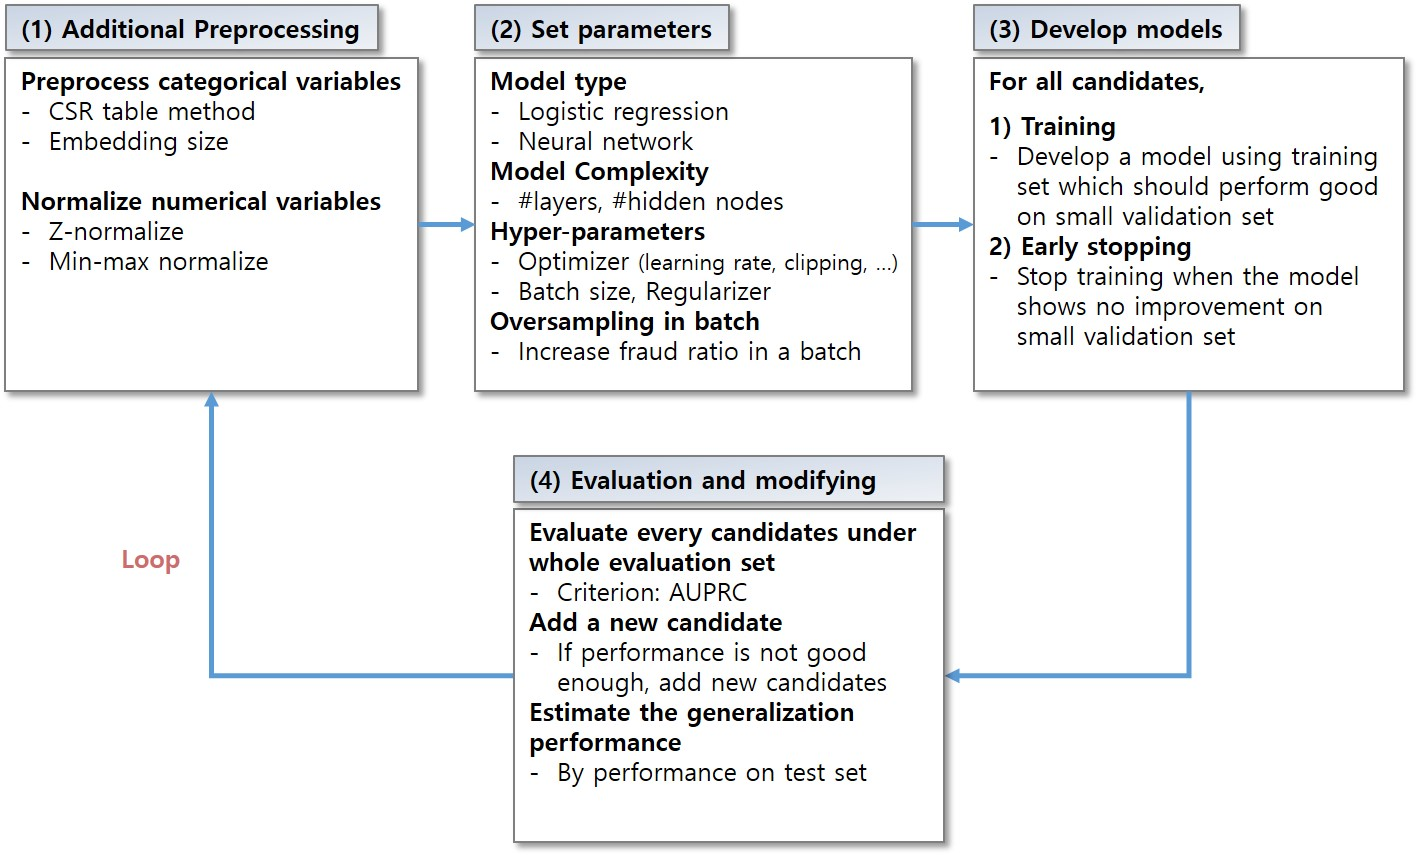
\includegraphics[width=0.9\textwidth]{[figure8]treatment-based_modeling.jpg}
   \vspace{-0.5cm}
   \caption{최적의 treatment-based scoring model을 탐색하는 방법}
   \vspace{0.5cm}
   \label{fig:treatment-based modeling}
\end{figure}

\section{Results}
\label{5}
\subsection{진료 내역 단위 모델링 결과}
\label{5.1}
각 진료과목에 대해서 진료 내역 단위 모델의 test set에서의 AUPRC값은 표~\ref{table: AUPRC}와 같다.
최적 모델 구조는 validation set에서의 AUPRC값을 기준으로 선택하였다.

% \usepackage{booktabs}
\begin{table}[]
    \centering
    \caption{Treatment-based model best AUPRC}
    \vspace{0.5cm}
    \label{table: AUPRC}
    \begin{tabular}{@{}lcc@{}}
    \toprule
                            & \multicolumn{1}{l}{Logistic regression} & \multicolumn{1}{l}{Proposed method} \\ \midrule
    Orthopedics             & 0.2415                                  & 0.5917                              \\ 
    Neurosurgery            & 0.4053                                  & 0.7203                              \\ 
    Pediatrics              & 0.4441                                  & 0.7324                              \\ 
    Rehabilitation Medicine & 0.3138                                  & 0.6314                              \\ 
    General Surgery         & 0.2966                                  & 0.6891                              \\ 
    Neurology               & 0.2464                                  & 0.6261                              \\ \bottomrule
    \end{tabular}
\end{table}




\subsection{기관 선정 효율성 평가 결과}
\label{5.2}
그림~\ref{fig:plot efficiency}는 Test set의 정형외과, 신경외과의 inpatient에 대해, 심사하는 청구명세서 수를 변화시키면서, 기존 모델과 TFID모델로 전문 심사 대상 기관을 선정하였을 때, 실제 탐지한 조정 금액의 변화를 도식화한 것이다.
이 때, 표~\ref{table: relative efficiency 1}는 각각의 경우에 대해서 relative efficiency의 값을 산출한 것이다.

그림~\ref{fig:plot efficiency}의 a)는 정형외과 입원환자의 청구명세서 심사량에 따른 실제 조정 금액의 변화를 나타낸다.
전문 심사할 수 있는 청구명세서가 전체의 80\%로 한정되어 있다고 하자.
이 때, 기존 모델 score로 전문 심사 대상 기관을 선정하였을 때, 심사 대상으로 선정된 기관의 수는 340개, TFID score 기관을 선정하였을 때, 선정된 기관의 수는 220개이다.
해당 기관의 총 청구명세서를 심사하였을 때, TFID score가 큰 기관을 선정할 경우, 기존 모델로 선정할 때 보다 1.09배 많은 금액을 조정할 수 있다는 것이다.
즉, 심사할 수 있는 청구명세서가 전체의 80\%만 심사한다고 할 때, TFID score로 전문 심사 대상 기관을 선정하는 것이 이 기존 선정 방법보다 1.09배 효율적이라는 의미이다.
마찬가지로, 심사할 수 있는 청구명세서가 60\%일 때, 1.13배, 40\%일 때 1.26배만큼 TFID가 더 효율적이라는 의미이다.

\begin{figure}[h]
   \centering
   \vspace{0.5cm}
   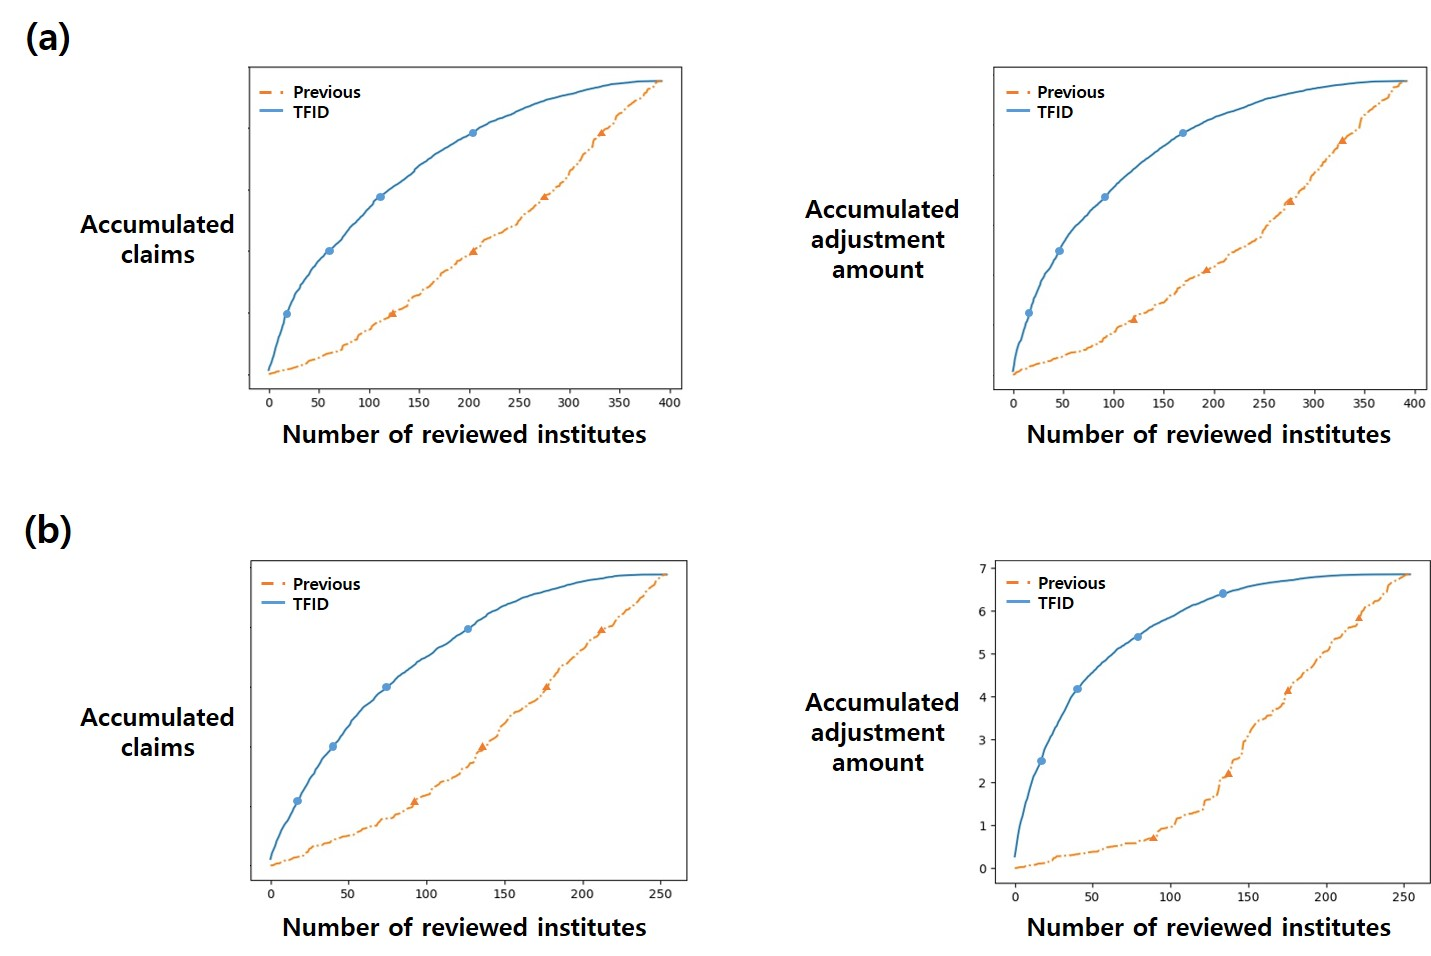
\includegraphics[width=0.9\textwidth]{[figure9]plot_efficiency.jpg}
   \vspace{-0.5cm}
   \caption{진료 과목별 누적 청구 명세서와 누적 조정 금액. 각 point들은 총 청구명세서의 20\%, 40\%, 60\%, 80\% 지점을 나타내며, 각 지점에서 기존 모델에서의 누적 조정 금액 대비 TFID 모델 사용 시 누적 조정 금액의 비율이 relative efficiency이다. (a):Orthopedics, (b): Neurosurgery}
   \vspace{0.5cm}
   \label{fig:plot efficiency}
\end{figure}


% \usepackage{booktabs}
\begin{table}[]
    \centering
    \caption{relative efficiency at the test set}
    \vspace{0.5cm}
    \label{table: relative efficiency 1}
    \begin{tabular}{@{}lccccc@{}}
    \toprule
    Reviewed claim ratio    & 0.2  & 0.4  & 0.6  & 0.8  & Max  \\ \midrule
    Orthopedics             & 1.02 & 1.26 & 1.13 & 1.09 & 1.34 \\
    Neurosurgery            & 3.33 & 1.91 & 1.26 & 1.14 & 3.50 \\
    Pediatrics              & 1.95 & 2.10 & 2.10 & 1.19 & 2.10 \\
    Rehabilitation medicine & 1.24 & 1.13 & 1.10 & 1.19 & 1.50 \\
    General surgery         & 1.61 & 1.23 & 1.21 & 1.17 & 1.61 \\
    Neurology               & 0.87 & 1.18 & 1.09 & 1.23 & 1.76 \\ \bottomrule
    \end{tabular}
\end{table}

\begin{table}[]
    \centering
    \caption{Precision@k at the test set (Previous model / TFID)}
    \vspace{0.5cm}
    \label{table: precision@k 1}
    \begin{tabular}{@{}lccccc@{}}
    \toprule
    Insitutuion ratio       & 0.1       & 0.2       & 0.3       & 0.4       & 0.5       \\ \midrule
    Orthopedics             & 0.00/0.70 & 0.05/0.82 & 0.16/0.84 & 0.24/0.92 & 0.37/0.90 \\
    Neurosurgery            & 0.00/0.77 & 0.06/0.90 & 0.08/0.88 & 0.14/0.87 & 0.29/0.92 \\
    Pediatrics              & 0.00/0.75 & 0.43/1.00 & 0.30/1.00 & 0.50/0.93 & 0.65/0.94 \\
    Rehabilitation medicine & 0.09/0.73 & 0.43/0.71 & 0.42/0.90 & 0.57/0.90 & 0.63/0.90 \\
    General surgery         & 0.38/0.94 & 0.38/0.81 & 0.47/0.87 & 0.51/0.95 & 0.59/0.91 \\
    Neurology               & 0.25/0.75 & 0.46/0.79 & 0.51/0.91 & 0.55/0.87 & 0.60/0.88 \\ \bottomrule
    \end{tabular}
\end{table}


표~\ref{table: relative efficiency 1}는 진료 과목별로 심사하는 청구명세서 비율을 다르게 하면서 relative efficiency값의 변화를 나타낸 것이다.
여기서 Max는 relative efficiency 값이 최대일 때의 심사 비율을 나타낸다.
모든 진료과목에서 1보다 큰 값을 갖는 것을 볼 수 있으며, 이는 모든 진료과목에서 기존 방법보다 더 효율적이라는 것을 의미한다.
또한, 이는 대체로 심사하는 청구명세서 비율이 작을 때, 큰 값을 갖는 경향이 있다.
이는 TFID모델이 실제 조정 금액이 높은 기관들을 더 잘 detect한다는 것을 의미한다.
이는 기관 단위 전문 심사  대상 기관들 중, 조정 금액으로 sorting하였을 때, 기존 모델과 TFID모델의 Precision@k 값을 나타낸 표~\ref{table: precision@k 1}에 더 잘 나타나 있다.
여기서, 진료 과목마다 병원의 수가 다르기 때문에, 기관수가 아닌 기관 비율을 변화시켜가면서 값을 측정하였다.

\subsection{TFID모델의 검증}
\label{5.3}
TFID방법은 진료 내역에 대해서 인공신경망이 산출한 결과인 fraudulent score와 각 진료 내역의 청구 금액을 곱하고, 그리고 이들을 기관의 모든 내역서에 대해서 합산하여, 기관의 fraudulent score를 산출하는 방식이다.
이러한 특징으로 인해, TFID score는 기관의 총 청구 금액에 비례하는 경향을 갖는다.
만약, 각 진료 내역에 대한 score term이 없었다면, TFID score는 단순히 기관의 총 청구 금액과 같고, 이는 전문 심사 대상 기관을 단순히 총 청구 금액이 많은 기관들을 선정하는 것과 같은 결과이다.
그러나, TFID model은 score term이 포함됨으로서 위와 같이 단순한 방식으로 전문 심사 대상 기관을 선정하지 않는다.
이를 증명하기 위해, 총 조정 금액을 기준으로 내림차순 정렬하였을 때 TFID score의 변화를 도식화하였다.
만약, 진료 단위 모델에서 산출한 score가 모델 선정에 영향을 끼치지 못한다면, TFID score도 단순 감소하게 된다.
그러나, 그림~\ref{fig:ADJ TFID wrt AMT}와 같이 감소하는 추세이긴 하지만, 단순 감소는 아닌 것을 봤을 때, TFID모델은 단순히 총 청구 금액이 많은 기관을 선정하는 것이 아님을 알 수 있다.

\begin{figure}[h]
   \centering
   \vspace{0.5cm}
   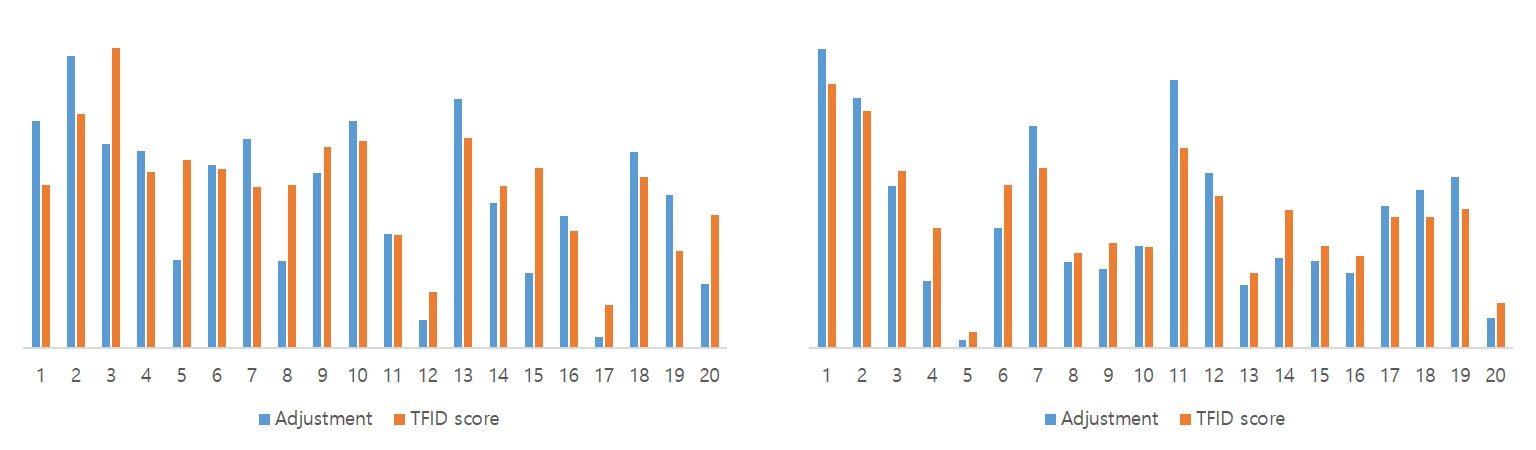
\includegraphics[width=0.9\textwidth]{[figure10]ADJ_TFID_wrt_AMT.jpg}
   \vspace{-0.5cm}
   \caption{진료 과목별 총 청구 금액을 기준으로 top 20개의 기관을 뽑았을 때, TFID score와 실제 조정 금액의 변화. 실제 청구 금액과 score나 실제 조정 금액은 내림차순으로 되는 경향이 있으나, 그렇지 않은 부분들이 더 많이 존재.(left):Orthopedics, (right): Neurosurgery }
   \vspace{0.5cm}
   \label{fig:ADJ TFID wrt AMT}
\end{figure}

% \usepackage{booktabs}
\begin{table}[]
    \centering
    \caption{relative efficiency comparison (other model / best model)}
    \vspace{0.5cm}
    \label{table: relative efficiency 2}
    \begin{tabular}{@{}lccccc@{}}
    \toprule
    Reviewed claim ratio    & 0.2       & 0.4       & 0.6       & 0.8       & Max       \\ \midrule
    Orthopedics             & 1.05/1.02 & 1.22/1.28 & 1.10/1.13 & 1.06/1.09 & 1.24/1.33 \\
    Neurosurgery            & 3.07/3.33 & 1.84/1.91 & 1.24/1.26 & 1.24/1.26 & 1.13/1.14 \\
    Pediatrics              & 1.95/1.95 & 2.10/2.10 & 2.10/2.10 & 1.19/1.19 & 2.10/2.10 \\
    Rehabilitation medicine & 0.98/1.24 & 0.89/1.13 & 1.03/1.10 & 1.04/1.19 & 1.33/1.50 \\
    General surgery         & 1.52/1.61 & 1.22/1.23 & 1.20/1.21 & 1.16/1.17 & 1.56/1.61 \\
    Neurology               & 0.61/0.87 & 0.97/1.18 & 1.09/1.09 & 1.22/1.23 & 1.22/1.76 \\ \bottomrule
    \end{tabular}
\end{table}

\begin{table}[]
    \centering
    \caption{Precision@k comparison (other model / best model)}
    \vspace{0.5cm}
    \label{table: precision@k 2}
    \begin{tabular}{@{}lccccc@{}}
    \toprule
    Insitutuion ratio       & 0.1       & 0.2       & 0.3       & 0.4       & 0.5       \\ \midrule
    Orthopedics             & 0.68/0.70 & 0.78/0.82 & 0.80/0.84 & 0.87/0.92 & 0.87/0.90 \\
    Neurosurgery            & 0.80/0.77 & 0.84/0.90 & 0.86/0.88 & 0.84/0.87 & 0.89/0.92 \\
    Pediatrics              & 0.75/0.75 & 0.86/1.00 & 0.90/1.00 & 0.93/0.93 & 0.94/0.94 \\
    Rehabilitation medicine & 0.64/0.73 & 0.62/0.71 & 0.81/0.90 & 0.81/0.90 & 0.86/0.90 \\
    General surgery         & 0.88/0.94 & 0.75/0.81 & 0.89/0.87 & 0.92/0.95 & 0.91/0.91 \\
    Neurology               & 0.75/0.75 & 0.83/0.79 & 0.86/0.91 & 0.83/0.87 & 0.86/0.88 \\ \bottomrule
    \end{tabular}
\end{table}

또한, 진료 내역 단위 모델이 잘 학습된 정도가 기관을 선정하는데 얼마나 많은 영향을 끼치는지 보이기 위해, 진료 내역 단위 모델에서 최적 모델이 아닌 임의의 다른 모델로 기관을 선정하였을 때, relative efficiency와 Precision@k값을 표~\ref{table: relative efficiency 2}와 표~\ref{table: precision@k 2}에 나타내었다.
두 결과 모두, 최적의 진료 단위 모델을 사용하여 기관을 선정했을 때보다, 결과가 좋지 않음을 보았을 때, 각 진료 내역을 잘 scoring하는 모델을 만드는 것이 기관을 선정할 때 영향을 미치는 것을 알 수 있다.

\subsection{2017년 데이터에 적용한 결과}
\label{5.4}


\begin{table}[]
    \centering
    \caption{manually reviewed in both 2016 and 2017)/manually reviewed in 2017}
    \vspace{0.5cm}
    \label{table: manual review in both years}
    \begin{tabular}{@{}lccc@{}}
    \toprule
    Department                                                        & \begin{tabular}[c]{@{}c@{}}Number of\\ institutions\end{tabular} & \begin{tabular}[c]{@{}c@{}}Number of\\ claims\end{tabular} & \begin{tabular}[c]{@{}c@{}}Number of\\ treatments\end{tabular} \\ \midrule
    Orthopedics                                                       & 259/327                & 280,083/291,031  & 24,274,388/24,593,125 \\ \midrule
    Neurosurgery                                                      & 101/133                & 77,247/80,758    & 5,875,745/6,138,625   \\ \midrule
    Pediatrics                                                        & 24/47                  & 14,706/19,239    & 1,029,135/1,291,242   \\ \midrule
    \begin{tabular}[c]{@{}l@{}}Rehabilitation\\ medicine\end{tabular} & 76/103                 & 75,922/77,498    & 3,646,965/3,728,786   \\ \midrule
    \begin{tabular}[c]{@{}l@{}}General\\ surgery\end{tabular}         & 128/182                & 31,214/32,790    & 2,121,534/2,209,681   \\ \midrule
    Neurology                                                         & 90/131                 & 28,902/31,191    & 1,915,349/2,025,883   \\ \bottomrule
    \end{tabular}
\end{table}

% \usepackage{booktabs}
\begin{table}[]
    \centering
    \caption{relative efficiency at the 2017 data}
    \vspace{0.5cm}
    \label{table: relative efficiency 3}
    \begin{tabular}{@{}lccccc@{}}
    \toprule
    Reviewed claim ratio    & 0.2  & 0.4  & 0.6  & 0.8  & Max  \\ \midrule
    Orthopedics             & 1.37 & 1.32 & 1.12 & 1.09 & 1.38 \\
    Neurosurgery            & 5.95 & 2.10 & 1.43 & 1.11 & 6.10 \\
    Pediatrics              & 1.00 & 3.45 & 2.10 & 1.70 & 3.53 \\
    Rehabilitation medicine & 1.60 & 1.14 & 1.21 & 1.12 & 1.80 \\
    General surgery         & 1.41 & 1.26 & 1.22 & 1.22 & 1.43 \\
    Neurology               & 0.82 & 0.99 & 0.98 & 1.15 & 1.39 \\ \bottomrule
    \end{tabular}
\end{table}

\begin{table}[]
    \centering
    \caption{Precision@k at the 2017 data (Previous model / TFID)}
    \vspace{0.5cm}
    \label{table: precision@k 3}
    \begin{tabular}{@{}lccccc@{}}
    \toprule
    Insitutuion ratio       & 0.1       & 0.2       & 0.3       & 0.4       & 0.5       \\ \midrule
    Orthopedics             & 0.00/0.66 & 0.06/0.71 & 0.14/0.72 & 0.24/0.78 & 0.37/0.81 \\
    Neurosurgery            & 0.00/1.00 & 0.00/0.76 & 0.00/0.81 & 0.07/0.88 & 0.24/0.82 \\
    Pediatrics              & 0.33/0.33 & 0.40/0.60 & 0.38/0.88 & 0.50/0.80 & 0.58/0.92 \\
    Rehabilitation medicine & 0.00/0.50 & 0.31/0.69 & 0.39/0.65 & 0.45/0.84 & 0.63/0.84 \\
    General surgery         & 0.38/0.69 & 0.35/0.77 & 0.46/0.74 & 0.48/0.71 & 0.58/0.80 \\
    Neurology               & 0.11/0.56 & 0.39/0.78 & 0.57/0.82 & 0.59/0.81 & 0.58/0.78 \\ \bottomrule
    \end{tabular}
\end{table}

본래 HIRA에서는 전년도 데이터를 기반으로 기관 단위 전문 심사 대상 기관을 선정하고, 선정된 기관을 이듬해 실제로 심사를 진행한다.
본 연구에서는 2016년의 training, validation set을 2016년의 데이터로 생각하고, 이를 원래 사용하던 모델과 TFID모델을 적용하여, 기관의 fraudulent score를 산출하고, 기관 단위 전문 심사 대상 기관을 선정하였다.
2016년 test set을 2017년의 data와 같이 생각하여, 앞에서 선정된 기관을 심사하였을 때, 심사의 효율성에 대해서 평가한 것이다.
이 절에서는 2016년 test set대신 2017년의 실제 심사 결과 data에 적용하였을 때, 심사의 효율성을 비교한다.
이를 위해 2016년과 2017년 모두 심사 결과 및 조정 금액에 대한 정보가 있는 데이터만을 활용해야 하는데, 이를 위해서 2016년과 2017년에 모두 기관 단위 전문 심사 대상이 되었던 기관에 대해서 결과를 비교한다.
(이 때, 진료 내역 단위 모델을 2017년의 데이터에 적용하여, 해당 모델의 정확성을 비교하는 방법도 있으나, 해당 연도 사이에 HIRA내부의 database관리 체계가 바뀌게 되어, 직접적인 비교가 어려웠기 때문에, 해당 task는 생략한다.)

2017년 데이터에서, 2016년과 2017년 모두 기관 단위 전문 심사 대상이 되었던 기관과, 해당 기관들의 청구 내역서 수, 총 진료 내역에 대한 정보는 표~\ref{table: manual review in both years}에 있다. 그리고, 심사 효율성에 대한 결과와 preicision@k, 값은 각각 표~\ref{table: relative efficiency 3}, 표~\ref{table: precision@k 3}와 같다. 실제로 앞의 결과와 유사하게 TFID모델이 기존의 모델보다 더 심사의 효율성이 높은 것을 볼 수 있고, 실제로 조정 금액이 높은 기관들을 잘 detect하는 것을 볼 수 있다.

\section{Conclusion and Future work}
\label{6}
본 연구에서는 최초로 의료 기관이 제출하는 가장 raw data인 진료 내역 단위의 데이터를 사용하여, 의료 기관이 환자에게 청구하는 billing pattern이 문제가 있는 정도를 나타내는 score를 산출하는 TFID모델을 제안하였다.
TFID모델은 두개의 단계로 나뉘어져 생성된다: (1)청구명세서 내의 개별 진료 내역이 문제가 있는지 여부를 scoring하는 인공신경망 기반의 모델을 구축한다.
(2): 각 개별 진료 내역의 진료 비용과, 해당 내역이 문제가 있는 정도를 나타내는 score를 곱한 뒤, 이를 기관별로 합산해서, 기관의 fraudulent한 정도를 나타내는 TFID score를 산출한다.
이 때, 모델링에 사용되는 데이터는 2016년 HIRA에 접수된 모든 청구명세서 데이터 중, 심사자들이 실제로 심사를 수행했던 진료 내역들이다. 

본 연구에서는 fraudulent billing pattern을 보이는 의료 기관을 선정하는데, 가장 raw data인 진료 내역 단위 데이터를 사용했다는 것에 큰 의의가 있다.
기존 연구들은 데이터에서 prescription per day, average per claim과 같이 기관 단위의 변수를 추출하고 모델링하는 것이 대부분이고, 기존에 HIRA에서 사용하던 모델도 이런 방법으로 기관을 선정하고 있었다.
이럴 경우, 기관 단위의 변수를 추출하면서, 개별 청구명세서나 진료 내역에서 얻을 수 있는 정보들을 많이 잃게 된다.
그러나, 본 연구에서는 진료 내역 단위 데이터를 활용함으로서 가장 raw data가 가지고 있는 정보들을 최대한 활용함으로서, fraudulent billing pattern을 보이는 의료 기관을 잘 선정할 수 있게 되었다.

모델이 fraudulent 기관을 잘 선정한다는 것은, 모델이 각 기관들의 fraudulent한 정도를 scoring한 결과가 실제로 조정이 된 금액과 비례하는 관계가 있다는 것을 의미한다.
이럴 경우, score가 전체 기관들 중, 모델의 score가 높은 일부 기관들에 대해서 심사를 진행하면, 조정 금액의 대부분을 detect 할 수 있다는 것이며, 이는 심사를 효율적으로 할 수 있다는 것을 의미한다.
2016년의 test set에서 TFID모델로 fraudulent 기관을 선정하였을 때, 기존에 사용하던 모델보다 효율적인 심사가 이루어진다는 것을 relative efficiency라는 measure를 도입하여 보였고, Precision@k 로 TFID score와 실제 조정 금액 간의 상관성이 높음을 보였다.
또한, 2017년의 실제 데이터에 이를 적용하였을 때, HIRA에서 기존에 사용하던 모델로 fraudulent 기관을 선정하여 심사를 하였을 때보다, TFID score를 기준으로 심사를 하였을 때가 심사의 효율성이 높음을 보였다.

그러나, HIRA에 수집되는 데이터의 특성상, 진료 내역 코드와 질병 내역 코드가 잘 매칭이 되어 있지 않다.
즉, 진료 내역을 발생시킨 원인 질병 간의 matching이 되어있지 않은 형태이다.
만약 이러한 causal관계가 잘 드러나있는 데이터를 활용한다면, 좀 더 정확한 진료 내역 단위 모델을 학습시킬 수 있을 것이다.
또한, 본 연구에서는 각 진료 내역 단위에 대해서 fraudulent score를 산출하는 진료 내역 단위 모델을 학습하였지만, 이 때, 청구 명세선 내의 다른 진료 내역 간의 관계를 고려하지 못한 형태이다.
실제로 심사자들이 청구 명세서를 심사할 때는, 청구 명세서의 개별 진료 내역 만을 따로 심사하는 것이 아니고, 해당 청구 명세서의 전체 진료 내역을 심사하고, 문제가 있는 진료 내역을 분류한다.
이와 같은 현재 모델의 한계점들은 추후에 보완한다면, 좀 더 정교한 scoring모델을 만들 수 있을 것이며, 심사의 효율성이 더 높아져, 사회 경제적 비용 낭비를 더 줄일 수 있을 것이다.

\bigskip
\textbf{Acknowledgement}

This work was supported by the BK21 Plus Program(Center for Sustainable and Innovative Industrial Systems, Dept. of Industrial Engineering, Seoul National University) funded by the Ministry of Education, Korea (No. 21A20130012638), the National Research Foundation(NRF) grant funded by the Korea government(MSIP) (No. 2011-0030814), and the Institute for Industrial Systems Innovation of SNU.

\bibliographystyle{unsrt}
\bibliography{ref}

\end{document}

